    \subsection{Descripci\'on}
    \par En este primer escenario se trabaj\'o sobre 4 distintas \textit{VLANs}
    de una misma terminal de trabajo en una red laboral.

    \par Estas cuatro diferentes VLANs nos dan 4 distintos dominios de colisi\'on,
    y cada VLAN tiene, claramente, un uso distinto (motivo por el cual los
    administradores de redes decidieron utilizarlos).

    \par Lo interesante aqu\'i es observar como distintos dominios tienen un
    vol\'umen completamente distinto de paquetes ARP seg\'un los dispositivos
    (estaciones de trabajo, servidores, computadoras, etc) y servicioes (Proxy,
    DNS, DHCP, etc) que pertenecen a la misma LAN.

    \par Se presenta a continuaci\'on una breve descripic\'on de cada una de las
    VLANS que fueron sniffeadas:

    \begin{LaTeXdescription}
        \item[Usuarios\label{itm:vlan10}]
            Esta VLAN se compone de todas las computadoras que se
            encuentran en el datacenter de la red laboral. Se entiende por
            datacenter como el edificio f\'isico donde se encuentran los servidores
            y todo el area de procesamiento central de distintos servicios de la
            red inform\'atica que se da a toda la red laboral. Es decir, en esta
            VLAN se encuentran todas las terminales ubicadas f\'isicamente en un
            edificio particular, donde la mayor\'ia de los usuarios hacen un uso
            avanzado de sus terminales.\\

        \item[Servidores\label{itm:vlan20}]
            Aqu\'i estamos observando la VLAN donde se conectan todos
            los servidores (enti\'endase por servidor como una terminal que ofrece
            uno o varios servicios particulares al resto de la red) de la red. La
            conectividad entre estos claramente estar\'a estrechamente relacionada
            con la interacci\'on que haya entre los servicios que provee cada
            \textit{server}.\\

        \item[Tel\'efonos\label{itm:vlan40}]
            Esta es la VLAN a la cual se conectan todos los
            dispositivos telef\'onicos de la red laboral. Tambi\'en aqu\'i hay
            ciertas computadoras que trabajan con \textit{telefon\'ia IP}.\\

        \item[Servidores+Usuarios\label{itm:vlan1}]
            Aqu\'i tenemos una VLAN en la que
            esperamos encontrar mucho tr\'afico, ya que es una vieja red que se
            utilizaba para todas las terminales y servidores de la red laboral antes
            de que se empezase a segmentar con diferentes VLANs y subredes (tarea que
            a\'un se encuentra en curso).\\

    \end{LaTeXdescription}

    \par Nuestro trabajo de \textit{sniffeo} en est\'as 4 redes mencionadas consisti\'o
    en utilizar la herramienta presentada en~\nameref{sec:tool} durante una semana entera,
    comenzando el domingo 14 y finalizando el s\'abado 20 de Septiembre del corriente a\~no.
    Dicha recolecci\'on de datos de la red fue realizada tambi\'en en un horario determinado,
    comenzando todos los d\'ias a las 7 y finalizando a las 18 horas.

    \subsection{An\'alisis de datos obtenidos}
    \par Antes de comenzar a exponer los distintos an\'alisis realizados sobre las redes
    ya descriptas, ser\'a util utilizar unas l\'ineas para unificar ciertos conceptos que
    se utilizar\'a n a continuaci\'on.

    \begin{LaTeXdescription}
        \item[Probabilidad Muestral] A la hora de referirnos a la probabilidad de cada
        s\'imbolo de las fuentes de datos analizadas, obtener su \textit{probabilidad
        real} es imposible, ya que el comportamiento de la fuente de datos es, \textit{%
        a prior\'i}, aleatorio. Por lo tanto, a la hora de asignar una probabilidad a cada
        s\'imbolo se utiliz\'o su probabilidad estad\'istica. Es decir, la cantidad de
        veces que se encontr\'o un determinado s\'imbolo sobre la cantidad total de mensajes
        que se capturaron.\\

        \item[Percentil 90] Dado que la fuentes de informaci\'on que se utilizaron contienen
        una gran cantidad de s\'imbolos, fue necesario trabajar con el percentil 90 en lugar
        de la totalidad de la informaci\'on, ya que m\'as del 99\% de los s\'imbolos no
        tuvieron, en conjunto, m\'as del 10\% de probabilidad.\\

    \end{LaTeXdescription}

    %-------------------------------------------------------------------------------------

    \subsubsection{VLAN de~\nameref{itm:vlan10}}
\par En una primera instancia, el primer resultado visible que se puede obtener es la
entrop\'ia de ambas fuentes de datos:

\begin{table}[!h]
\centering
  \begin{tabular}{c c}
    Fuente de Datos & Entrop\'ia \\
    \hline\hline
    Direcci\'on Origen & 3.87546 \\
    Direcci\'on Destino & 6.50272 \\
    \hline\hline
    \#IPs de las Fuentes & 4428\\
    \#Paquetes Capturados & 825978\\
    \hline
    \end{tabular}
  \bigskip
  \caption{Entrop\'ia VLAN \nameref{itm:vlan10}}
\end{table}

\par Hasta el momento, s\'olo con este \'unico dato, mucho no se puede decir sobre la red.
Pasaremos entonces analizar cada fuente por separada:


\subsubsection*{\underline{VLAN \nameref{itm:vlan10}: Fuente Origen}}\label{subsubsec:vlan10_src}

\begin{figure}[!ht]
    \centering
    \includegraphics[width=0.5\textwidth]{escenario_1/vlan10/vlan10_src_bars_percentile90}
    \caption{Probabilidades VLAN \nameref{itm:vlan10} - Fuente Origen}
    \label{fig:vlan10_src_prob_per90}
\end{figure}

\par Observemos la figura \ref{fig:vlan10_src_prob_per90}. La misma se compone de 2
datos analizados sobre los resultados obtenidos. Por 
un lado, en el eje \textit{x} se tienen ordenadas, de mayor a menor, todas las IPs de la
fuente de datos seg\'un su probabilidad muestral. Los s\'imbolos en cuesti\'on (IPs) no
son expuestos en la gr\'afica a\'un ya que se solapar\'ian y har\'ian ilegible al gr\'afico.
En lugar de ello se expuso la cantidad de IPs que hay hasta cada punto marcado del eje%
\footnote{Donde dice \textit{5, 10, 15...}, se tienen de izquierda a derecha 5 IPs, 10
IPs, etc.}. 

\par En rojo tenemos la probabilidad muestral de los s\'imbolos (que por el orden impuesto
ir\'a obviamente decreciendo).

\par Por \'ultimo, en azul se puede ver la l\'inea de progreso de probabilidad acumulada.
En cada s\'imbolo del eje \textit{x}, la l\'inea azul nos indica cual es la sumatoria de
las probabilidades de todos los s\'imbolos (comenzando por el de mayor probabilidad) hasta
dicho punto.\\

\par As\'i pues, podemos observar que se llega al percentil 90 con tan solo los 27 s\'imbolos
de mayor probabilidad de la fuente. Es decir que menos del 0.01\% de los s\'imbolos aparecen
en nuestra fuente de datos con un 90\% de probabilidad.

\par Visto esto, ya nos interesa pasar a analizar de que IPs exactamente estamos hablando.
Como se vi\'o, en el an\'alisis lo m\'as determinante parecer\'ia ser aquellas IPs inclu\'idas
dentro del percentil 90. Las mismas se presentan a continuaci\'on:

\begin{figure}[!ht]
    \centering
    \includegraphics[width=0.5\textwidth]{escenario_1/vlan10/vlan10_src_probabilities_with_labels}
    \caption{IPs VLAN \nameref{itm:vlan10} - Fuente Origen}
    \label{fig:vlan10_src_prob_ips}
\end{figure}

\par Se puede observar en la figura \ref{fig:vlan10_src_prob_ips} que las primeras 6 IPs parecer\'ian
ser las principales de la red en enviar paquetes ARP (recordemos que estamos viendo los resultados
de la fuente de origen, es decir, los paquetes ARP cuya direcci\'on origen es la que fue
analizanda). Claramente estas IPs ya son candidatas a tener en cuenta al buscar nodos importantes
de nuestra red, ya que claramente est\'an env\'iando m\'as paquetes ARP que el resto, aunque el
motivo nos sea desconocido.


\subsubsection*{\underline{VLAN \nameref{itm:vlan10}: Fuente Destino}}\label{subsubsec:vlan10_dst}
\par Pasamos ahora a visualizar en la figura \ref{fig:vlan10_dst_prob_per90} los datos obtenidos
en la misma red, pero en la fuente destino, es decir, las IP's a las que fueron enviados los
paquetes ARP (o, dicho de otra forma, aquellos nodos a cuyos paquetes estaban destinados).

\begin{figure}[!ht]
    \centering
    \includegraphics[width=0.5\textwidth]{escenario_1/vlan10/vlan10_dst_bars_percentile90}
    \caption{Probabilidades VLAN \nameref{itm:vlan10} - Fuente Destino}
    \label{fig:vlan10_dst_prob_per90}
\end{figure}

\par Nuevamente, se puede observar que se alcanza el percentil 90 de probabilidad de la
fuente con tan solo poco menos de 135 s\'imbolos (apr\'oximadamente representan un
0.03\% de la totalidad de IPs observadas en la fuente). Claramente, nos encontramos
nuevamente ante la situaci\'on de una red donde los destinos de los paquetes ARP
est\'an concentrados en unos pocos nodos. De hecho, no es casualidad que la cantidad
de personas que trabajan en esta red sean 70\footnote{Apr\'oximadamente}. Si se tienen
en cuenta algunos otras IPs que claramente no son de usuarios (posiblemente servidores)
y la posibilidad de usuarios con m\'as de una IP en la red\footnote{Interfases virtuales,
recordar que los \textit{hosts} de esta red son personal de un datacenter.}.

\par De hecho, si se observa con atenci\'on se podr\'a ver que en realidad, las primeras
50 IPs con mayor probabilidad conforman el percentil 80.

\par Observemos entonces, cuales son est\'as IPs que concentran la gran mayor\'ia
de la informaci\'on de nuestra fuente destino\footnote{En lugar de exponer la probabilidad
de las 135 IPs que componen el percentil 90, se tuvieron en cuenta las primeras 50 -percentil
80- dado que graficar tantos s\'imbolos har\'ia ilegible el gr\'afico y, a\'un m\'as importante
a\'un, a la hora de distinguir nodos importantes de la red, es muy probable que estos
se encuentren dentro de este percentil 80 que concentra tanta informaci\'on.}. Dicha informaci\'on
se presenta en la figura \ref{fig:vlan10_dst_prob_ips}.

\begin{figure}[!ht]
    \centering
    \includegraphics[width=0.5\textwidth]{escenario_1/vlan10/vlan10_dst_probabilities_with_labels}
    \caption{IPs VLAN \nameref{itm:vlan10} - Fuente Destino}
    \label{fig:vlan10_dst_prob_ips}
\end{figure}

\par En este \'ultimo gr\'afico podemos observar que dentro de las IPs que forman el percentil 80,
las 10 primeras IPs claramente componen la parte m\'as importante de la fuente. Es abrupta
la diferencia de las probabilidades, como se puede observar. As\'i pues, est\'as IPs que 
pareciesen ser muy solicitadas dentro de nuestra red, son claras candidatas a representar
nodos importantes.


\subsubsection*{\underline{VLAN \nameref{itm:vlan10}: Ambas Fuentes}}\label{subsubsec:vlan10_src_dst}
\par Toda la informaci\'on presentada hasta el momento nos permiti\'o identificar ciertas IPs
de la red (o s\'imbolos de la fuente) que seguramente son candidatos a representar algo notorio
o importante en la red \textit{sniffeada}. Pero a\'un no podemos llegar a conclusiones de la red,
dado que s\'olo obtivimos posibles IPs para dos fuentes distintas.

\par Para poder llegar a razonamientos coherentes sobre la red, debemos poder unir la informaci\'on
hasta ahora presentada de alguna manera. En primer instancia, es interesante observar las
relaciones entre las concentraciones de nodos de ambas fuentes (cantidad de IPs dentro del percentil
90/80 respecto de la totalidad de IPs de las fuentes) y las entrop\'ias:

\begin{table}[!h]
\centering
  \begin{tabular}{c c c c}
    Fuente& 
    Entrop\'ia & \begin{tabular}{@{}c@{}}Concentraci\'on \\ Percentil 90\end{tabular} 
    & \begin{tabular}{@{}c@{}}Concentraci\'on \\ Percentil 80\end{tabular}\\
    \hline\hline
    Origen & 3.87546 & 0.006\% & 0.002\%\\
    Destino & 6.50272 & 0.03\% & 0.015\%\\
    \hline\hline
    \end{tabular}
  \bigskip
  \caption{Concentraci\'on VLAN \nameref{itm:vlan10}}
  \label{tab:vlan10_concentracion}
\end{table}

\par Interesante como se ve el cuadro \ref{tab:vlan10_concentracion}, la \'unica nueva informaci\'on
que nos da es que claramente es que la incertidumbre de la fuente destino es mayor que la de la 
fuente destino. Es decir, mirando la concentraci\'on de los percentiles vemos que el 90\% de
probabilidades de la fuente destinoest\'a acumulado en un 0.03\% de los s\'imbolos de la fuente,
mientras que en la fuente origen est\'a a\'un m\'as concentrada. Esta concentraci\'on a nosotros,
dado nuestro objetivo, nos resulta \'util ya que nos permite reducir la cantidad de IPs que
probablemente cumplan con un rol importante dentro de la red.

\par As\'i pues llegamos a esta instancia con una reducci\'on de unas 160 IPs (entre ambas fuentes)%
\footnote{Se filtraron las IPs que componen los percentiles 90 de ambas fuentes.}
entre las cuales seguramente se encuentren los hosts importantes de la red \textit{sniffeada}. Se
presenta entonces a continuaci\'on un digrafo de la red entera, se\~nalando estas IPs candidatas.

\par Dado el gran tama\~no del \textit{dataset} (muchos nodos y muy denso en ejes\footnote{%
aproximadamente unos 4400 nodos con 12000 ejes}), se decidi\'o filtrar un poco m\'as los datasets
con alg\'un concepto intuitivo: si durante 77 horas de captura, un cierto par ordenado de direcciones
IP de un paquete ARP no se captur\'o m\'as de 500 veces, podemos asumir que dicho par no aporta
mucha informaci\'on, ya que se trata de informaci\'on espor\'adica que nos dan las fuentes de
datos.

\begin{figure*}[!t]
    \centering
    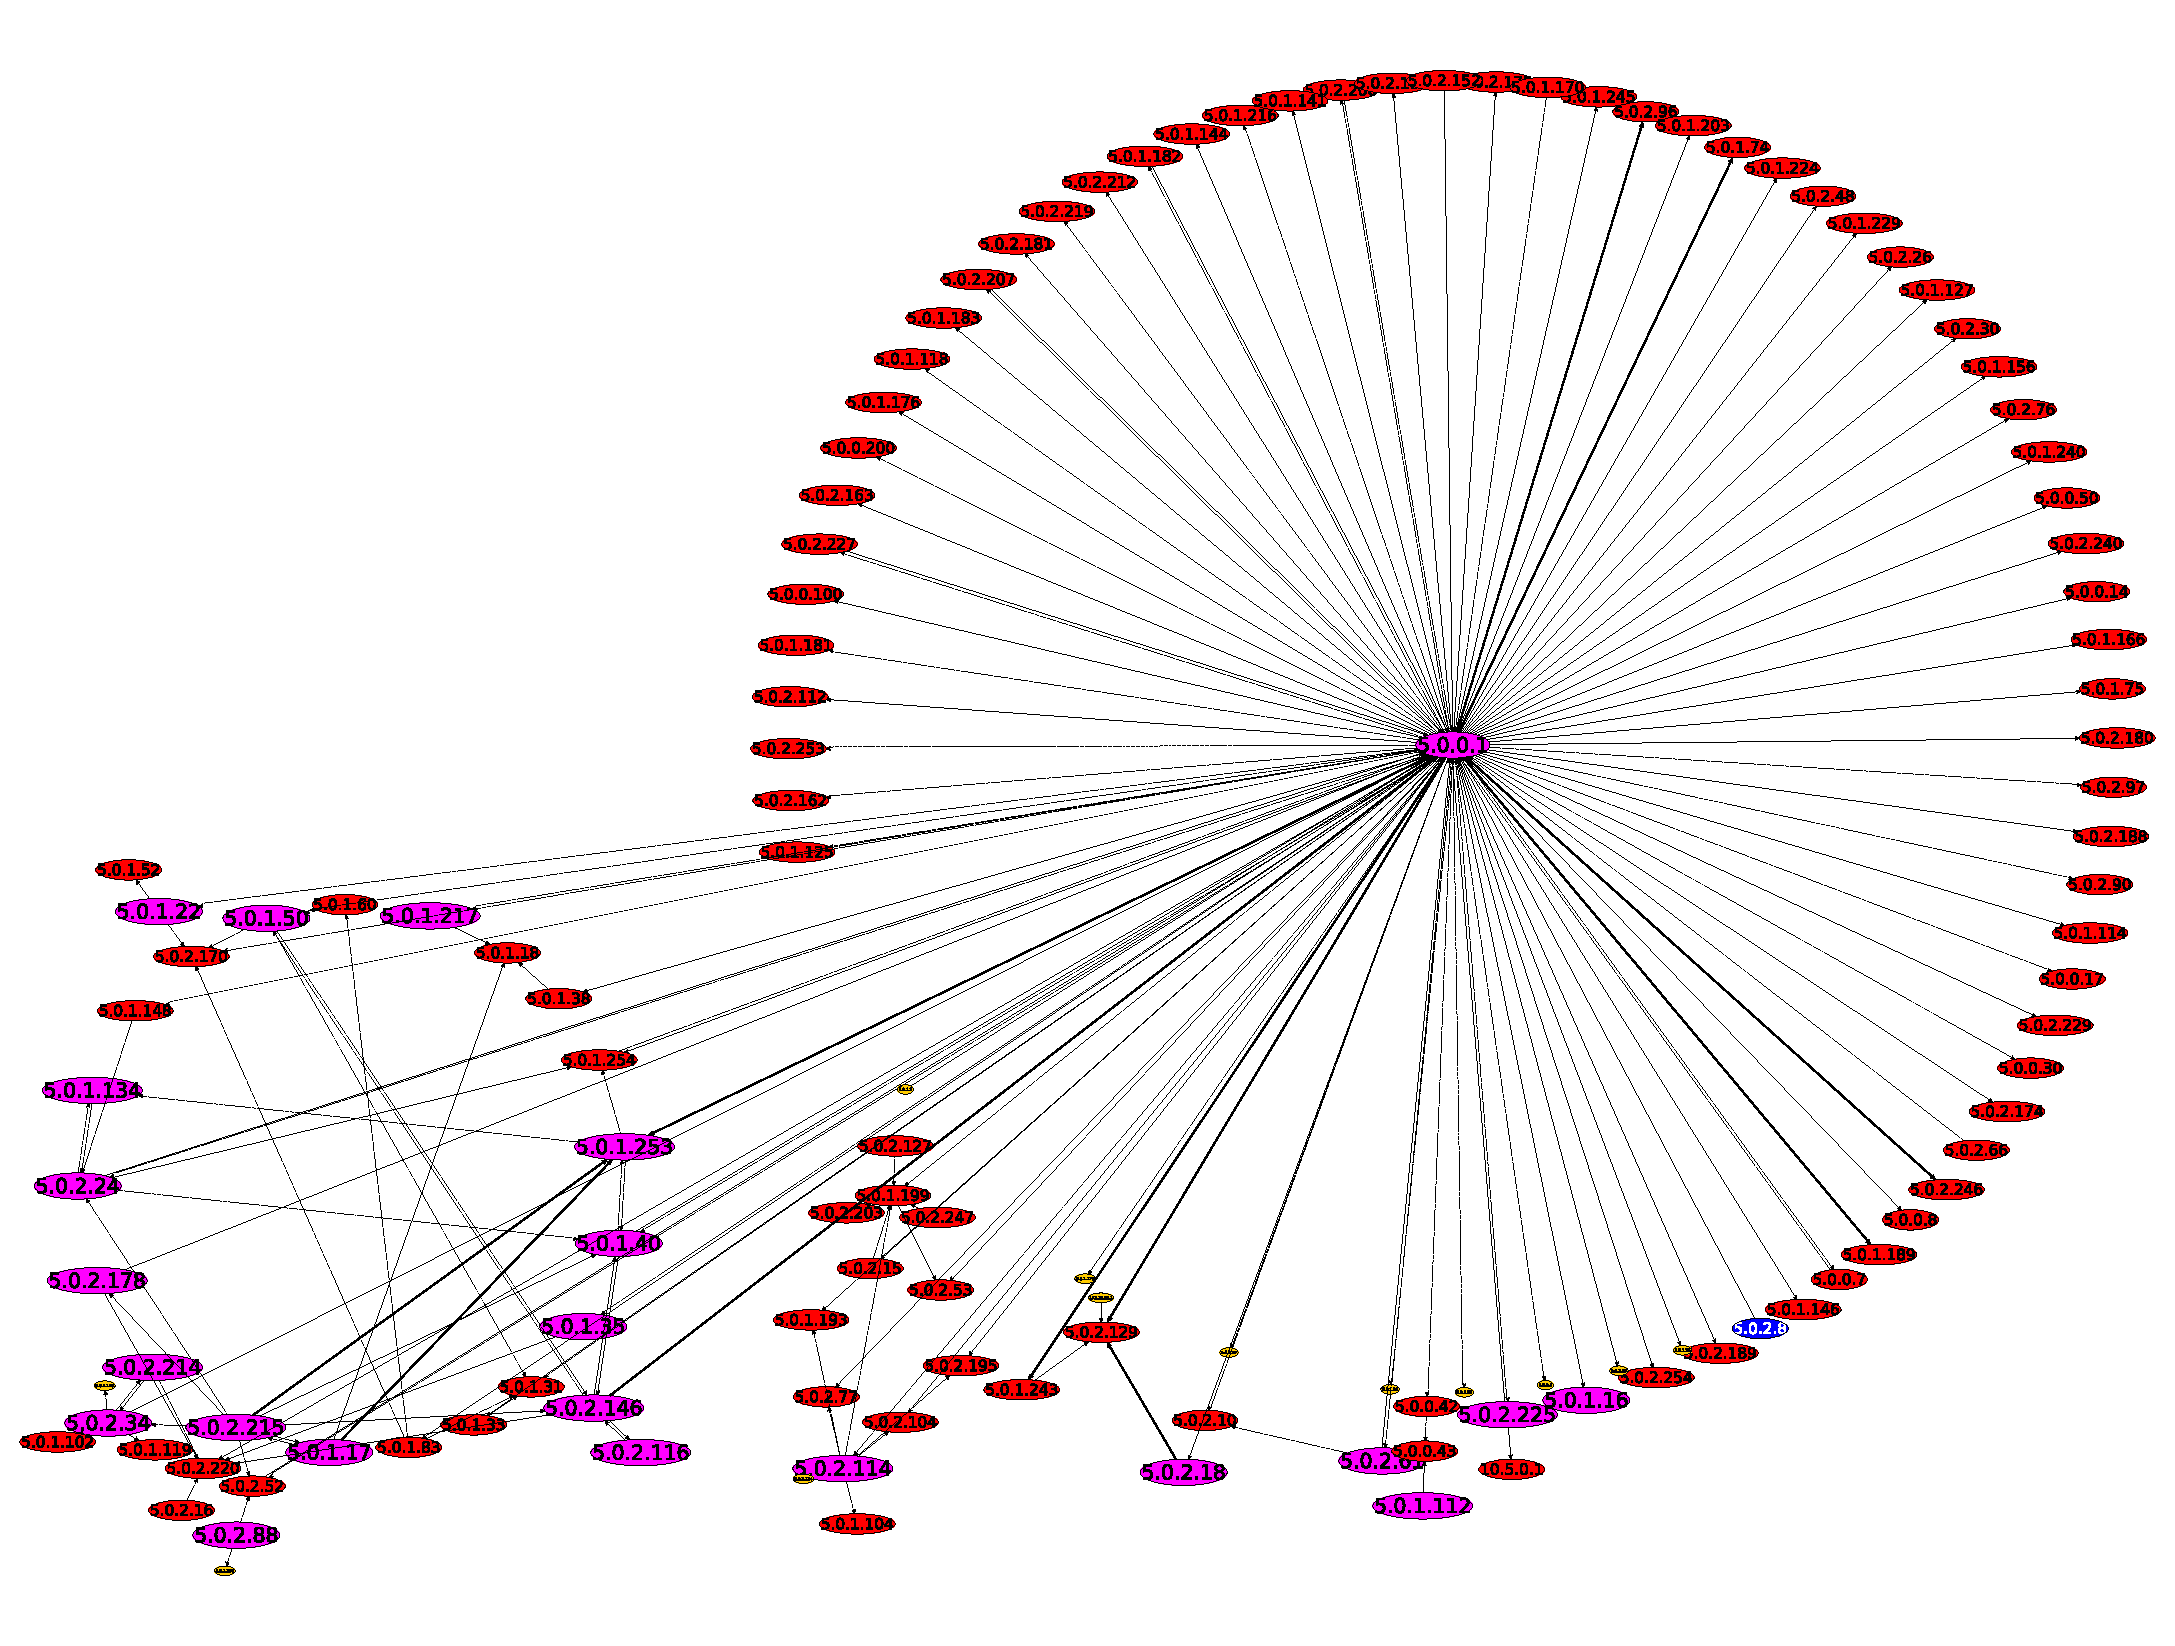
\includegraphics[width=\textwidth]{img/graph/escenario_1/vlan10/vlan10_500toEnd}
    \caption{Grafo VLAN \nameref{itm:vlan10}}
    \label{fig:vlan10_grafo}
\end{figure*}

\par En el grafo en cuesti\'on (figura \ref{fig:vlan10_grafo}) se colorearon los nodos
siguiendo la siguiente l\'ogica:

\begin{LaTeXdescription}
    \item[Rojo] Son los nodos que forman parte del percentil 90 de la fuente de
    direcciones de destino.\\

    \item[Azul] Son los nodos que forman parte del percentil 90 de la fuente de 
    direcciones de origen.\\

    \item[Violeta] Son las direcciones que forman parte del percentil 90 de ambas
    fuentes de direcciones.\\

\item[Ejes] Los ejes fuero formateados de manera tal que representacen el peso de los
    ejes. Es decir, la cantidad de paquetes con las direcciones origen y destino (o nodos)
    conectados por cada eje. A menor peso, la l\'inea ser\'a menos gruesa y hasta
    punteada, mientras que en el caso contrar\'i el eje ir\'a ganado grosor.\\

\end{LaTeXdescription}

\par Como se observa, el grafo parece indicar un flujo de paquetes ARP amplio desde
el nodo del centro hacia la gran mayor\'ia de los dem\'as nodos. En dicho nodo (que se
ampl\'ia en la figura \ref{fig:vlan10_grafo_centro}), puede notarse una afluencia
balanceada en cuanto a flechas entrando (direcci\'on destino) y flechas saliendo
(direcci\'on origen\footnote{No por nada dicha IP est\'a marcada con el color
\textit{violeta}.}). A su vez, si nos concentramos en los grosores de los ejes,
veremos que tambi\'en se encuentra enviando paquetes ARP con la misma (al menos
en una primera vista del gr\'afo) \textit{intensidad} con la que los recibe
por los demas nodos de la red.

\begin{figure}
    \centering
    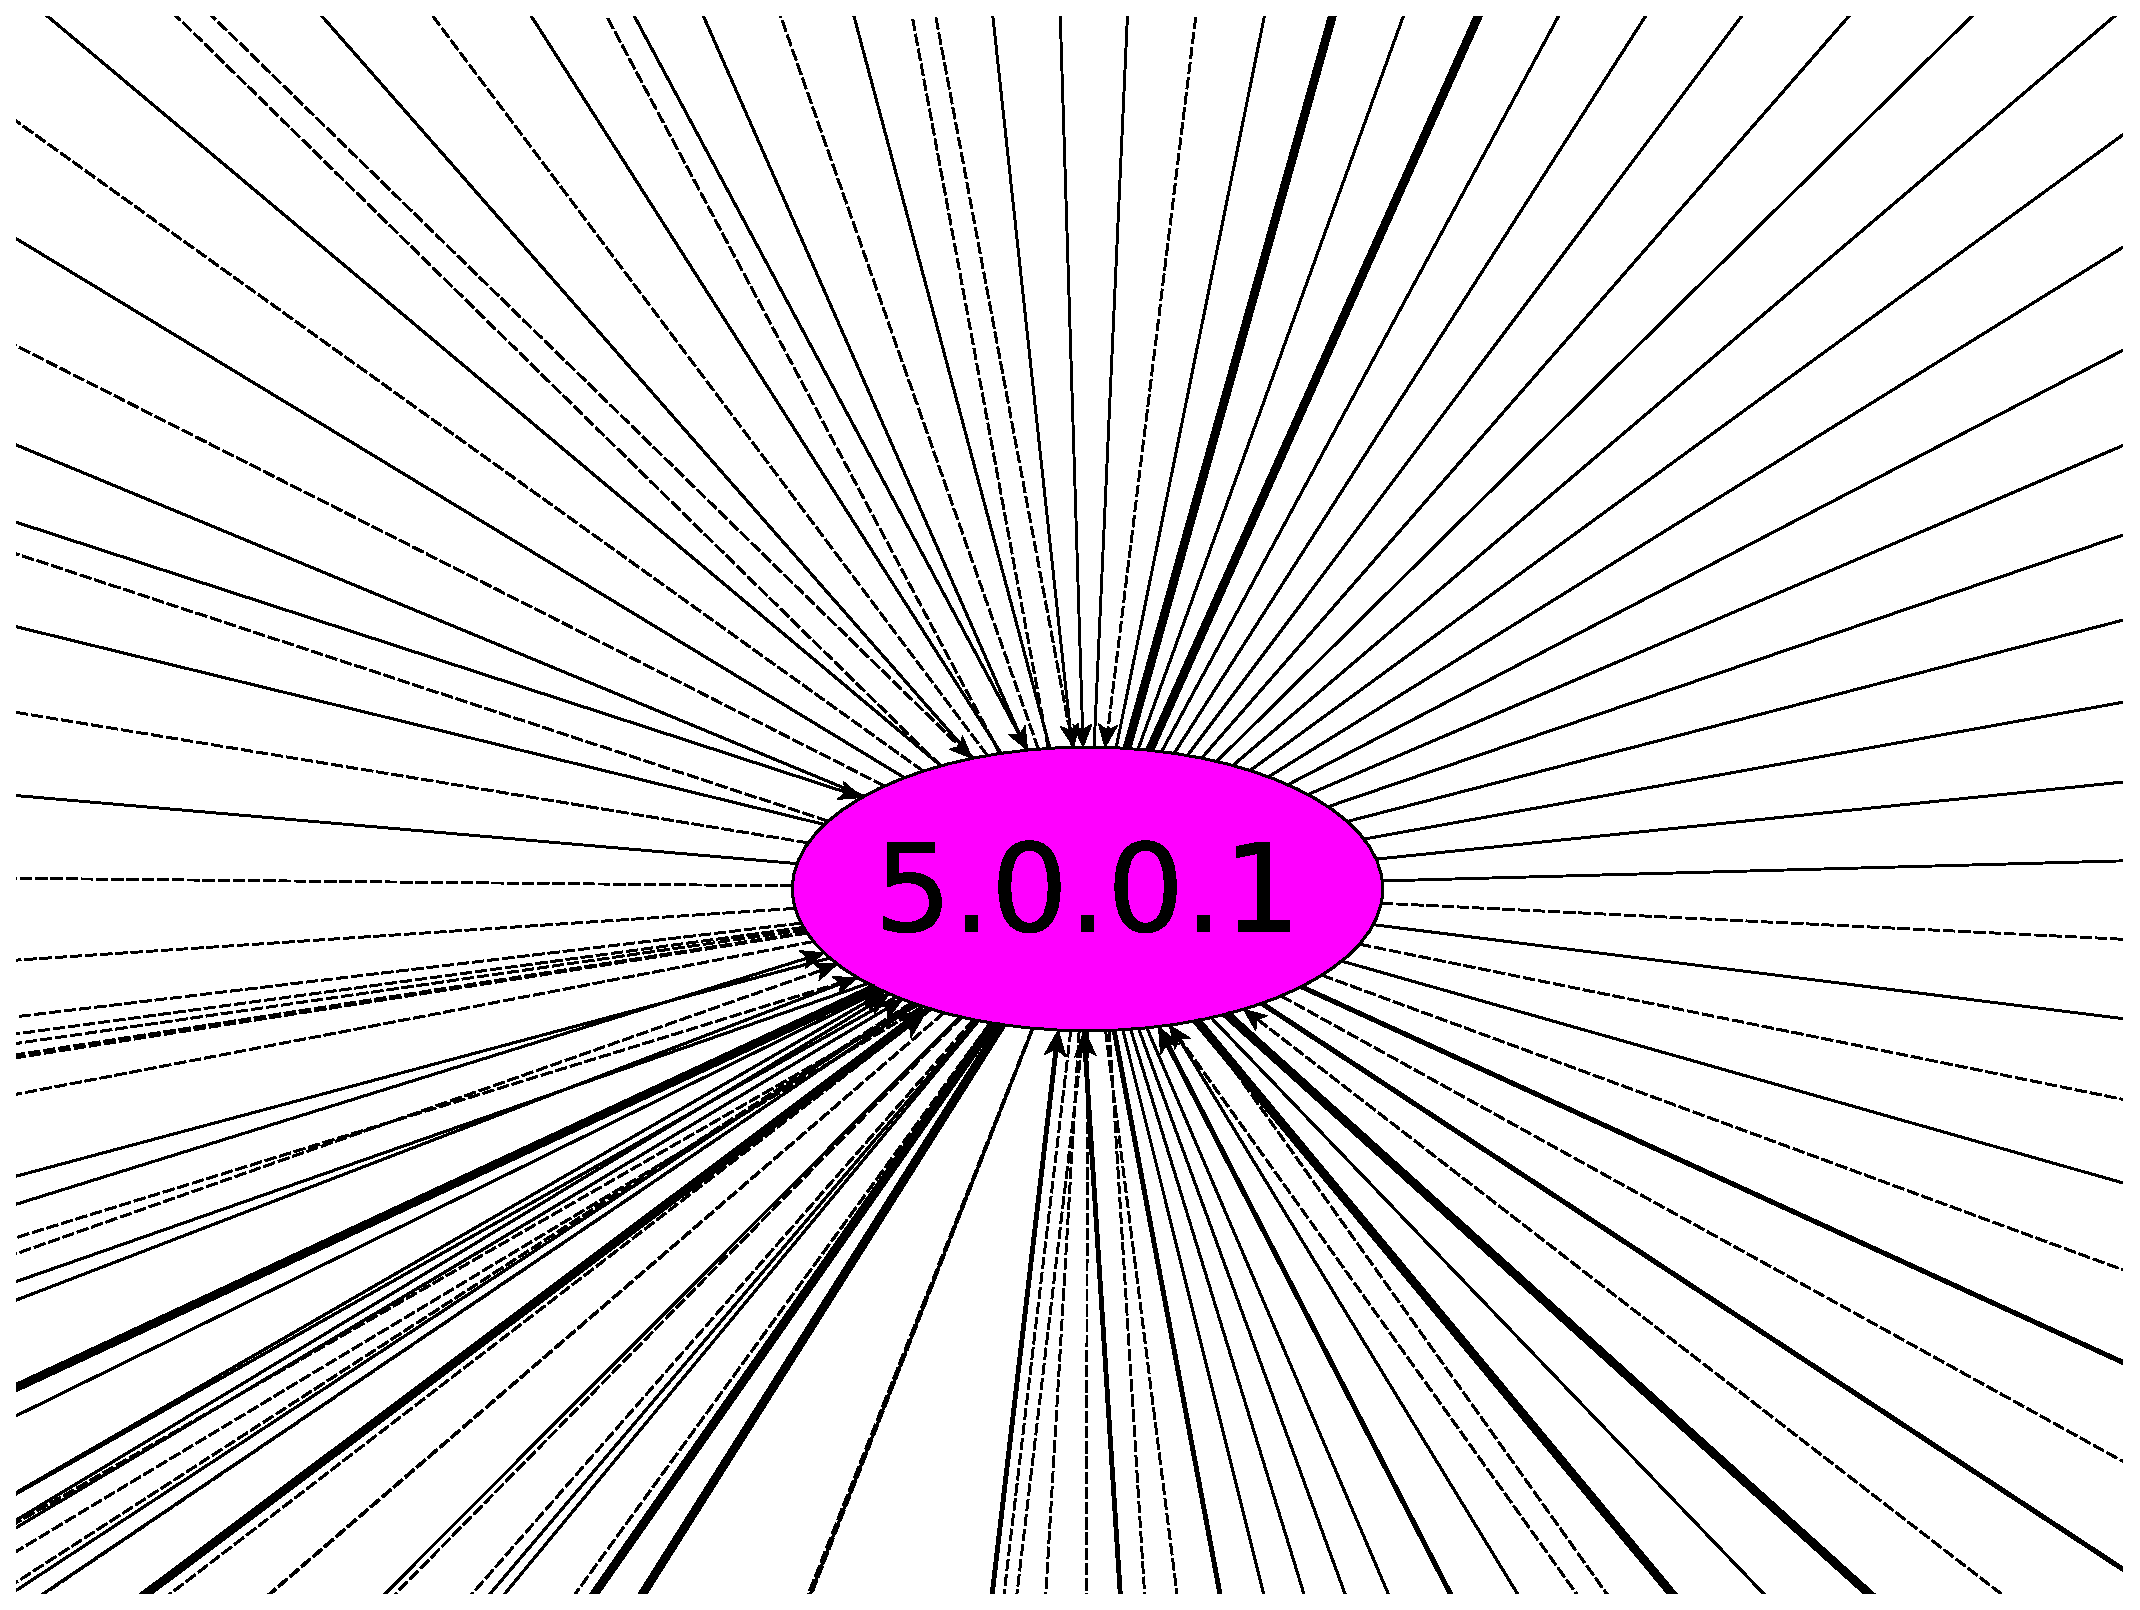
\includegraphics[width=0.5\textwidth]{img/graph/escenario_1/vlan10/vlan10_500toEnd_centro}
    \caption{Grafo VLAN \nameref{itm:vlan10} - Centro}
    \label{fig:vlan10_grafo_centro}
\end{figure}

\par Por \'ultimo, se observa una \textit{subregi\'on} en la zona izquierda donde varios
nodos parecer\'ieran estar env\'iandoso paquetes entre s\'i con bastante regularidad. A
\textit{prior\'i} estos parecer\'ian ser los nodos m\'as activos de la red durante el
transcurso de la semana. Se puede observar dicha zona en la figura \ref{fig:vlan10_grafo_inf}:

\begin{figure}
    \centering
    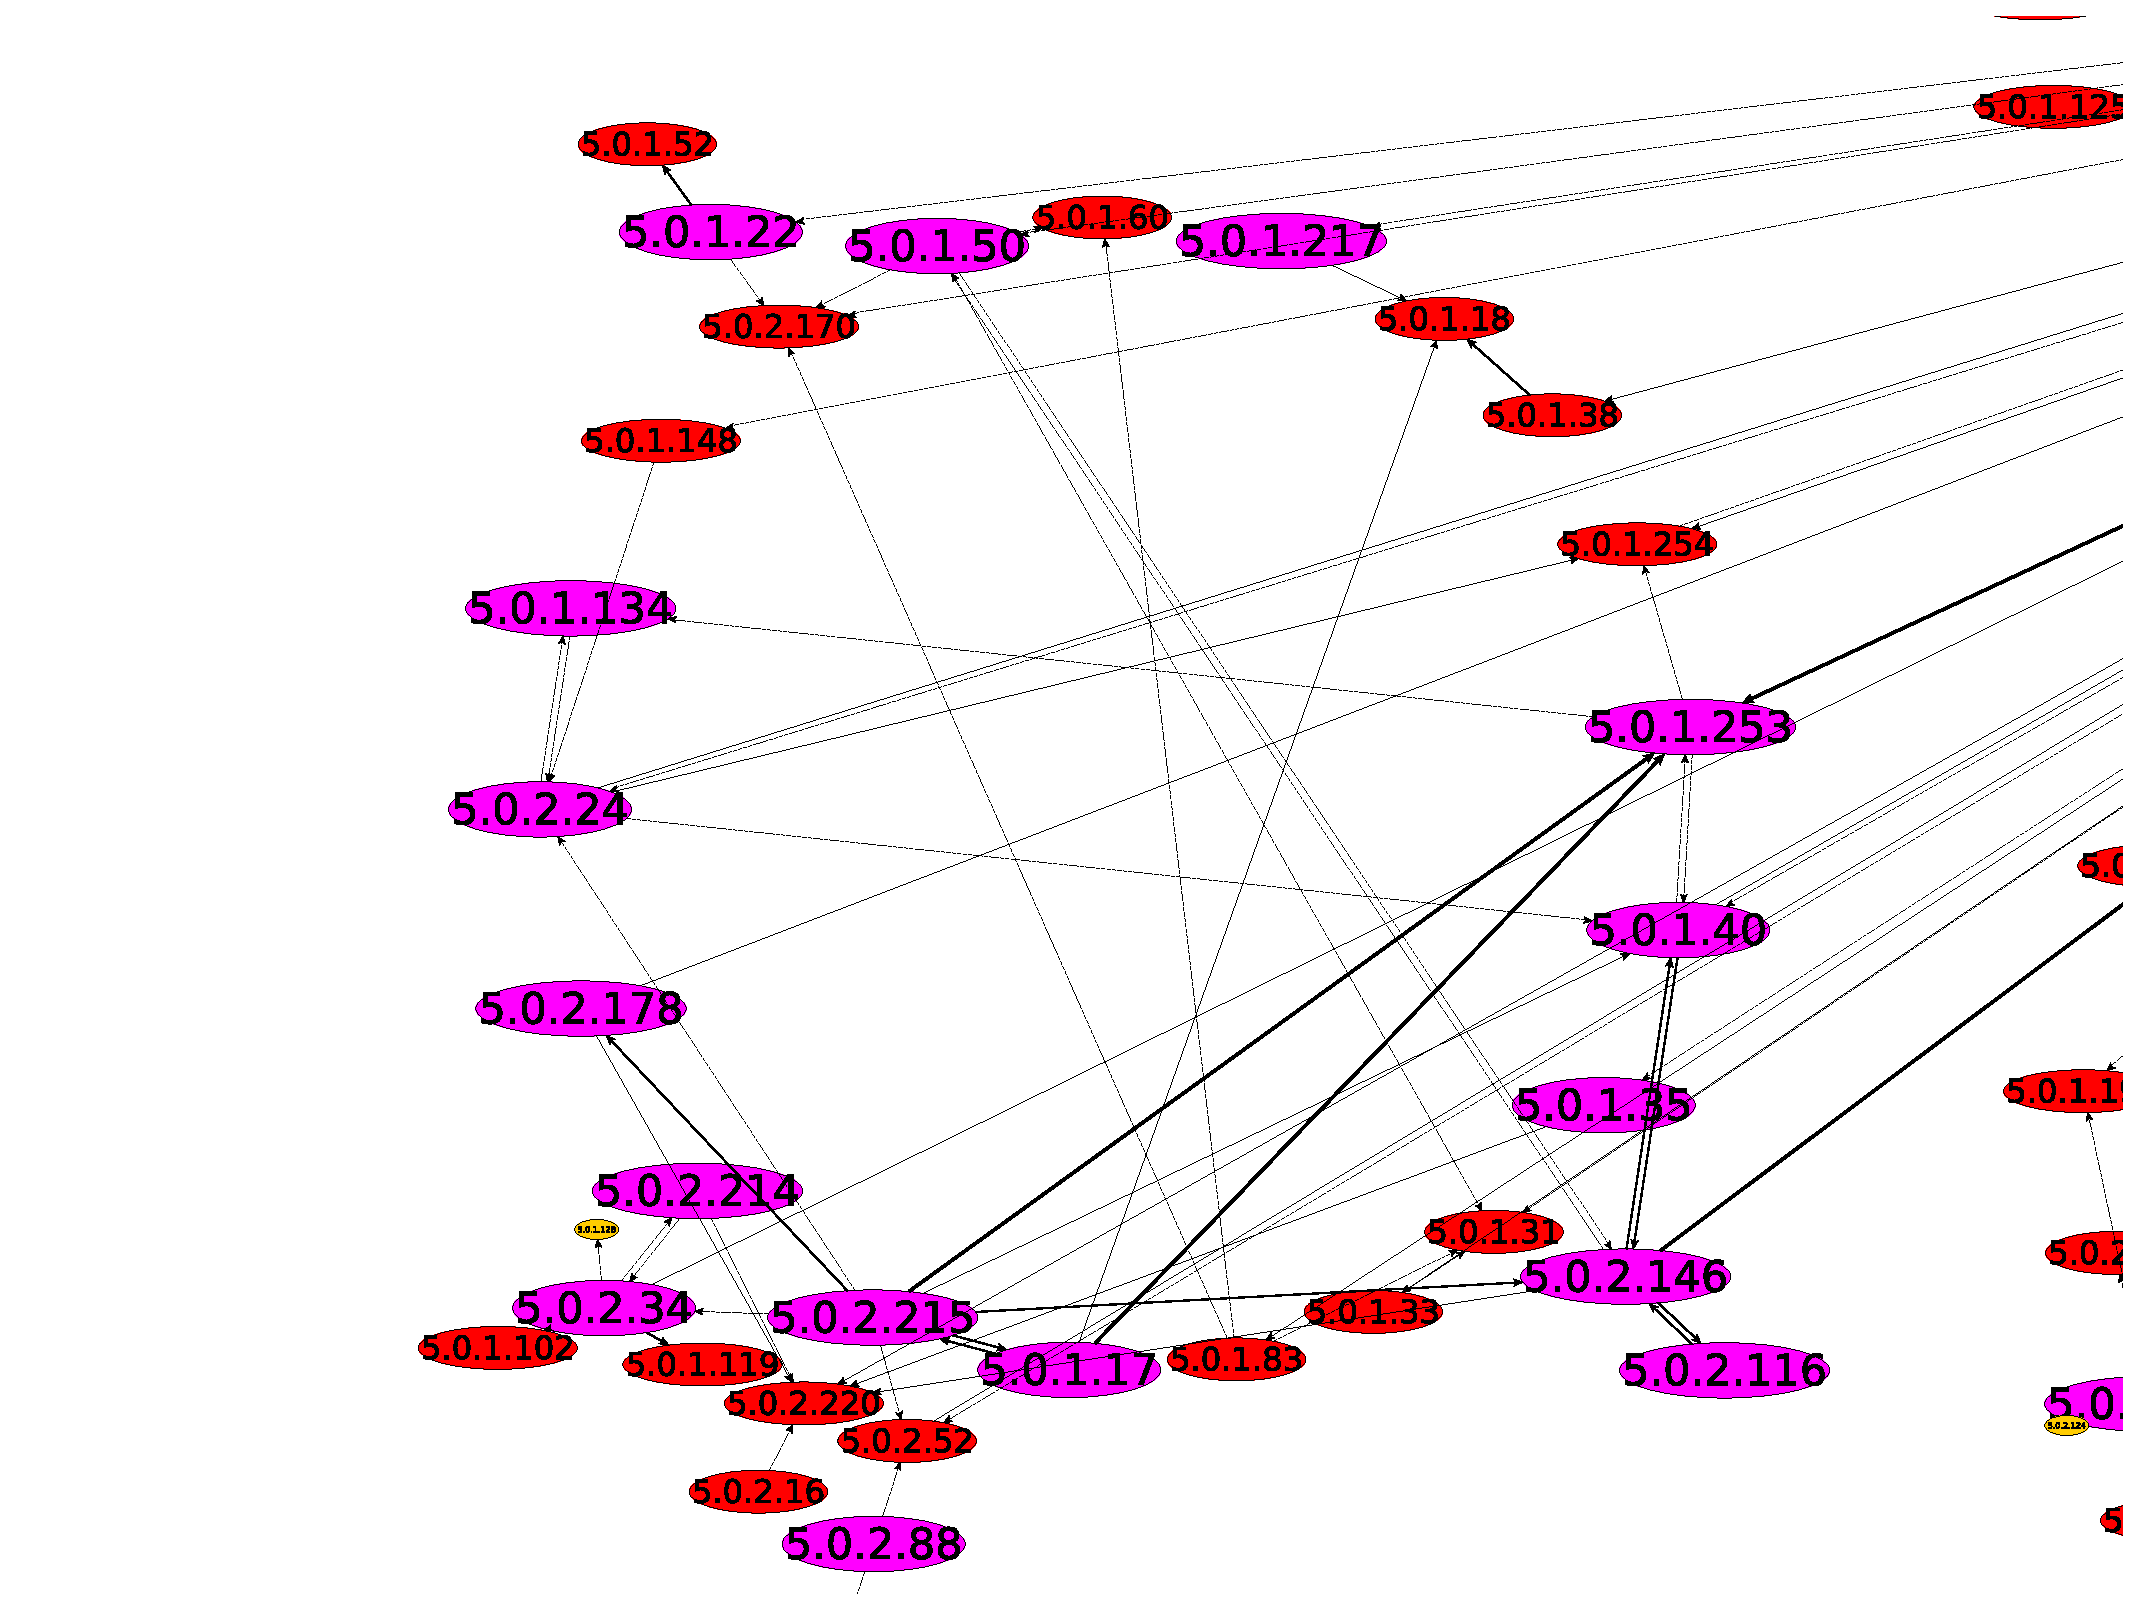
\includegraphics[width=0.5\textwidth]{img/graph/escenario_1/vlan10/vlan10_500toEnd_inf}
    \caption{Grafo VLAN \nameref{itm:vlan10} - Zona activa}
    \label{fig:vlan10_grafo_inf}
\end{figure}

\par En dicha regi\'on se puede ver que a pesar de la elevada actividad cruzada de paqutes
ARP entre los nodos, no hay nodo tan concurrido como el \textit{5.0.0.1}, el cual se
vi\'o en detalle hace tan solo unos momentos.


\subsubsection*{\underline{VLAN \nameref{itm:vlan10}: Conclusiones}}\label{subsubsec:vlan10_conclusiones}
\par Podemos concluir que claramente la direcci\'on \textit{5.0.0.1} es una
direcci\'on importante de la red. Se v\'io como aparece entre las direcciones con mayor
probabilidad tanto en la fuente de direcciones origen as\'i como destino, y se nota
en el grafo que es de entre los nodos con mayor probabilidad aquel que tiene la mayor
interacci\'on (en cuanto a cantidad) con el resto de los \textit{hosts} de la redes.

\par Este comportamiento es sumamente similar al comportamiento que tendr\'ia un equipo
encargado de \textit{routear} la red LAN hac\'ia otras redes, debido a la gran cantidad
de equipos que piden por su direcci\'on \textit{MAC} dentro de la VLAN.

\par Quiz\'as valga mencionar que de hecho hay otros nodos importantes en la red. Se
puede ver en la figura \ref{fig:vlan10_grafo_inf} como hay tres direcciones que se env\'ian
pedidos ARP con bastante frecuencia: \textit{5.0.1.253, 5.0.1.17, 5.0.2.15 y 5.0.246}.
No parecer\'ia ser casualidad que a todas estas IPs les haya correspondido el color
violeta en el grafo. Claramente la interaccion que tienen entre s\'i (m\'as all\'a de la
que tienen con los dem\'as nodos) parecer\'ia ser suficente, por las caracter\'isticas
de los ejes, para tener una alta probabilidad en ambas fuentes de s\'imbolos. Claramente
esto ser\'ia un dato de inter\'es para el administrador de la red, debido a que quiz\'as
estos equipos est\'an env\'iando paquetes broadcast en el dominio de colisi\'on sin
que haya necesidad.


    \subsubsection{VLAN de~\nameref{itm:vlan20}}
\par Habiendo ya pasado por el proceso de analizar una VLAN, nos encontramos en una
situaci\'on mucho m\'as concisa. En esta VLAN esperamos encontrar mucho menos tr\'afico
que en la anterior. Este razonamiento se debe a que esta es una red de servidores, con
lo cual se espera estar tomando datos de un ambiente mucho m\'as administrado, con
menos varianza de las terminales que se prenden/apaguan conectan/desconectan.

\par Estas caracter\'isticas del entorno nos hacen razonar tambi\'en que al ser
servidores con mucha menos manipulaci\'on, con las conexiones dentro de la LAN
seguramente mucho m\'as estables ya que nadie est\'a usando est\'as terminales
para \textit{salir} a internet o utilizandolas activamente con servicios que
deban salir a otra red salvo para la comunicaci\'on con los usuarios que se conectan
a los mismos.

\par As\'i pues, pasamos a los datos concretos de nuestro an\'alisis:

\begin{table}[!h]
\centering
  \begin{tabular}{c c}
    Fuente de Datos & Entrop\'ia \\
    \hline\hline
    Direcci\'on Origen & 3.01743 \\
    Direcci\'on Destino & 5.71059 \\
    \hline\hline
    \#IPs de las Fuentes & 2051\\
    \#Paquetes Capturados & 874806\\
    \hline
    \end{tabular}
  \bigskip
  \caption{Entrop\'ia VLAN \nameref{itm:vlan20}}
  \label{tab:vlan20_entropia}
\end{table}

\par Curiosamente, los resultados aqu\'i obtenidos nos dan una cantidad de paquetes
similar a la de la VLAN \nameref{itm:vlan10}. Compararemos estos resultados m\'as
adelante en la secci\'on \ref{sec:escenario1_supl}.


\subsubsection*{\underline{VLAN \nameref{itm:vlan20}: Fuente Origen}}\label{subsubsec:vlan20_src}
\par Pasamos ahora a visualizar las distintas probabilidades que nos d\'a esta fuente de
datos.

\begin{figure}[!ht]
    \centering
    \includegraphics[width=0.5\textwidth]{escenario_1/vlan20/vlan20_src_bars_percentile90}
    \caption{Probabilidades VLAN \nameref{itm:vlan20} - Fuente Origen}
    \label{fig:vlan20_src_prob_per90}
\end{figure}

\par El resultado inmediato que se puede observar aqu\'i es la poca cantidad de IPs
requeridas para componer el percentil 90. Se ver\'a m\'as adelante que la concentraci\'on
de la informaci\'on en esta VLAN es mucho mayor que en el caso anterior. Se puede
ver con claridad que con tan solo con las 5 IPs de mayor probabilidad muestral se obtiene
la probabilidad acumulada del 90\% de la fuente. A\'un as\'i, vale la pena mencionar
nuevamente el dato expresado en la tabla \ref{tab:vlan20_entropia}, donde se puede
observar que la cantidad de IPs/S\'imbolos que nos di\'o la fuente fue extensamente
mayor.

\par Esto ya parecer\'ia estar indicando que en la red hay muy pocas terminales que
env\'ian paquetes ARP, al menos con una frecuencia comparable al caso de la VLAN
ya analizada.


\subsubsection*{\underline{VLAN \nameref{itm:vlan20}: Fuente Destino}}\label{subsubsec:vlan20_dst}
\par Veamos ahora que pasa con las otras terminales a la hora de responder a los
paquetes ARP. La pregunta que nos realizamos es si esas 5 terminales que acaparaban
todo el tr\'afico de env\'io de paquetes ARP es entre ellas, distribu\'ido entre
las dem\'as direcciones de la LAN o si simplemente son paquetes ARP env\'iados para
monitorear la red, en cuyo caso ir\'ian dirigidos a IPs inexistentes.

\begin{figure}[!ht]
    \centering
    \includegraphics[width=0.5\textwidth]{escenario_1/vlan20/vlan20_dst_bars_percentile90}
    \caption{Probabilidades VLAN \nameref{itm:vlan20} - Fuente Destino}
    \label{fig:vlan20_dst_prob_per90}
\end{figure}

\par Notoriamente en este caso se puede observar como para alcanzar el percentil
90 se necesitan de algo menos que las 1200 direcciones IPs con mayor probabilidad
muestral. Ya esto nos da la pauta, a diferencia de lo que ve\'iamos observando
hasta este momento, de que en este entorno la fuente de direcciones destino
no est\'a tan concentrada. De hecho, parecer\'ia haber una \'unica IP que
es destinatario de m\'as de alg\'un paquete ARP, dandonos a entender que no es
una coincidencia impulsada, quiz\'as, por el tama\~no de la red el hecho de que
sea la \'unica IP de esta fuente de datos con una probabilidad no desestimable.

\begin{figure}[!ht]
    \centering
    \includegraphics[width=0.5\textwidth]{escenario_1/vlan20/vlan20_dst_probabilities_with_labels}
    \caption{IPs VLAN \nameref{itm:vlan20} - Fuente Destino}
    \label{fig:vlan20_dst_prob_ips}
\end{figure}


\par Ya llegados a estas instancias, nos resulta interesante ver la siguiente tabla
y como contrasta con la del caso anterior:

\begin{table}[!h]
\centering
  \begin{tabular}{c c c c}
    Fuente& 
    Entrop\'ia & \begin{tabular}{@{}c@{}}Concentraci\'on \\ Percentil 90\end{tabular} 
    & \begin{tabular}{@{}c@{}}Concentraci\'on \\ Percentil 80\end{tabular}\\
    \hline\hline
    Origen & 3.01743 & 0.0024\% & 0.0014\%\\
    Destino & 5.71059 & 0.573\% & 0.183\%\\
    \hline\hline
    \end{tabular}
  \bigskip
  \caption{Concentraci\'on VLAN \nameref{itm:vlan10}}
  \label{tab:vlan20_concentracion}
\end{table}

\par Los n\'umeros aqu\'i ya nos est\'an diciendo mucho sobre la red. La baja entro\'ia
de la fuente de origen nos comunica que estamos ante una fuente de datos bastante
predecible. De hecho, esto luego se ve confirmado por la baja concentraci\'on de 
s\'imbolos que componen el percentil 90 y 80. Claramente con muy pocas direcciones
ya se tiene una gran probabilidad acumulada de la fuente, sabiendo entonces que seguramente,
si hay un paquete ARP, poder indicar 6 direcciones sobre 2051 con una probabilidad muestral
del 90\%.

\par Por lo contrar\'io, la fuente destino es ya bastante m\'as impredecible. Si bien su
entrop\'ia no es alta (al menos comparada con los otros casos ya expuestos), vemos una
concentraci\'on considerable (respecto de la fuente de origen) en el percentil 90. Pero
observando la figura \ref{fig:vlan20_dst_prob_ips}, podemos ver que en realidad, hay
una direcci\'on particular que tiene casi un 25\% de probabilida de surgir de esta fuente, pero
ocurre que todas las dem\'as direcciones tienen una probabilidad muy baja. Por lo tanto,
sabemos que existe una \'unica IP en realidad que podr\'ia llegar a ser esperada con cierta
justificaci\'on, pero es todo lo que podemos decir de este dominio de colisi\'on.


\subsubsection*{\underline{VLAN \nameref{itm:vlan20}: Ambas Fuentes}}\label{subsubsec:vlan20_src_dst}
\par A diferencia de la VLAN de \nameref{itm:vlan10}, aqu\'i ya pudimos obtener varios
resultados interesantes y bastante expl\'icitos sobre el comportamiento de las fuentes
de informaci\'on analizados. No obstante, es interesante verificar como se compone
el gr\'afo de esta fuente, en parte para confirmar las hip\'otesis planteadas sobre
el funcionamiento de la red y tambi\'en para verificar si no hay alg\'un dato
o caractar\'istica que no pueda ser visto mediante las probabilidades ya expuestas.

\par En el grafo que se presenta a continuaci\'on se utilizan las mismas reglas de coloreo
y de grosores ya explicadas en la secci\'on \ref{subsubsec:vlan10_src_dst}. Al igual
que en el caso anterior, desestimamos aquellos ejes que no tuvieran un peso
superior a 70 (en lugar de 500 del caso anterior, ya que esta VLAN contiene muchas
menos direcciones IP y mucho menos tr\'afico ARP tambi\'en). La justificaci\'on subyacente
es la misma que antes: luego de 77 horas de captura de paquetes, si un servidor
trata de obtener espor\'adicamente la \textit{MAC} de otra terminal, es un dato
que no nos suma a la topolog\'ia que tratamos de descubrir (ya que agregar\'a ejes
que ocurren con muy poca probabilidad).

\begin{figure*}[!t]
    \centering
    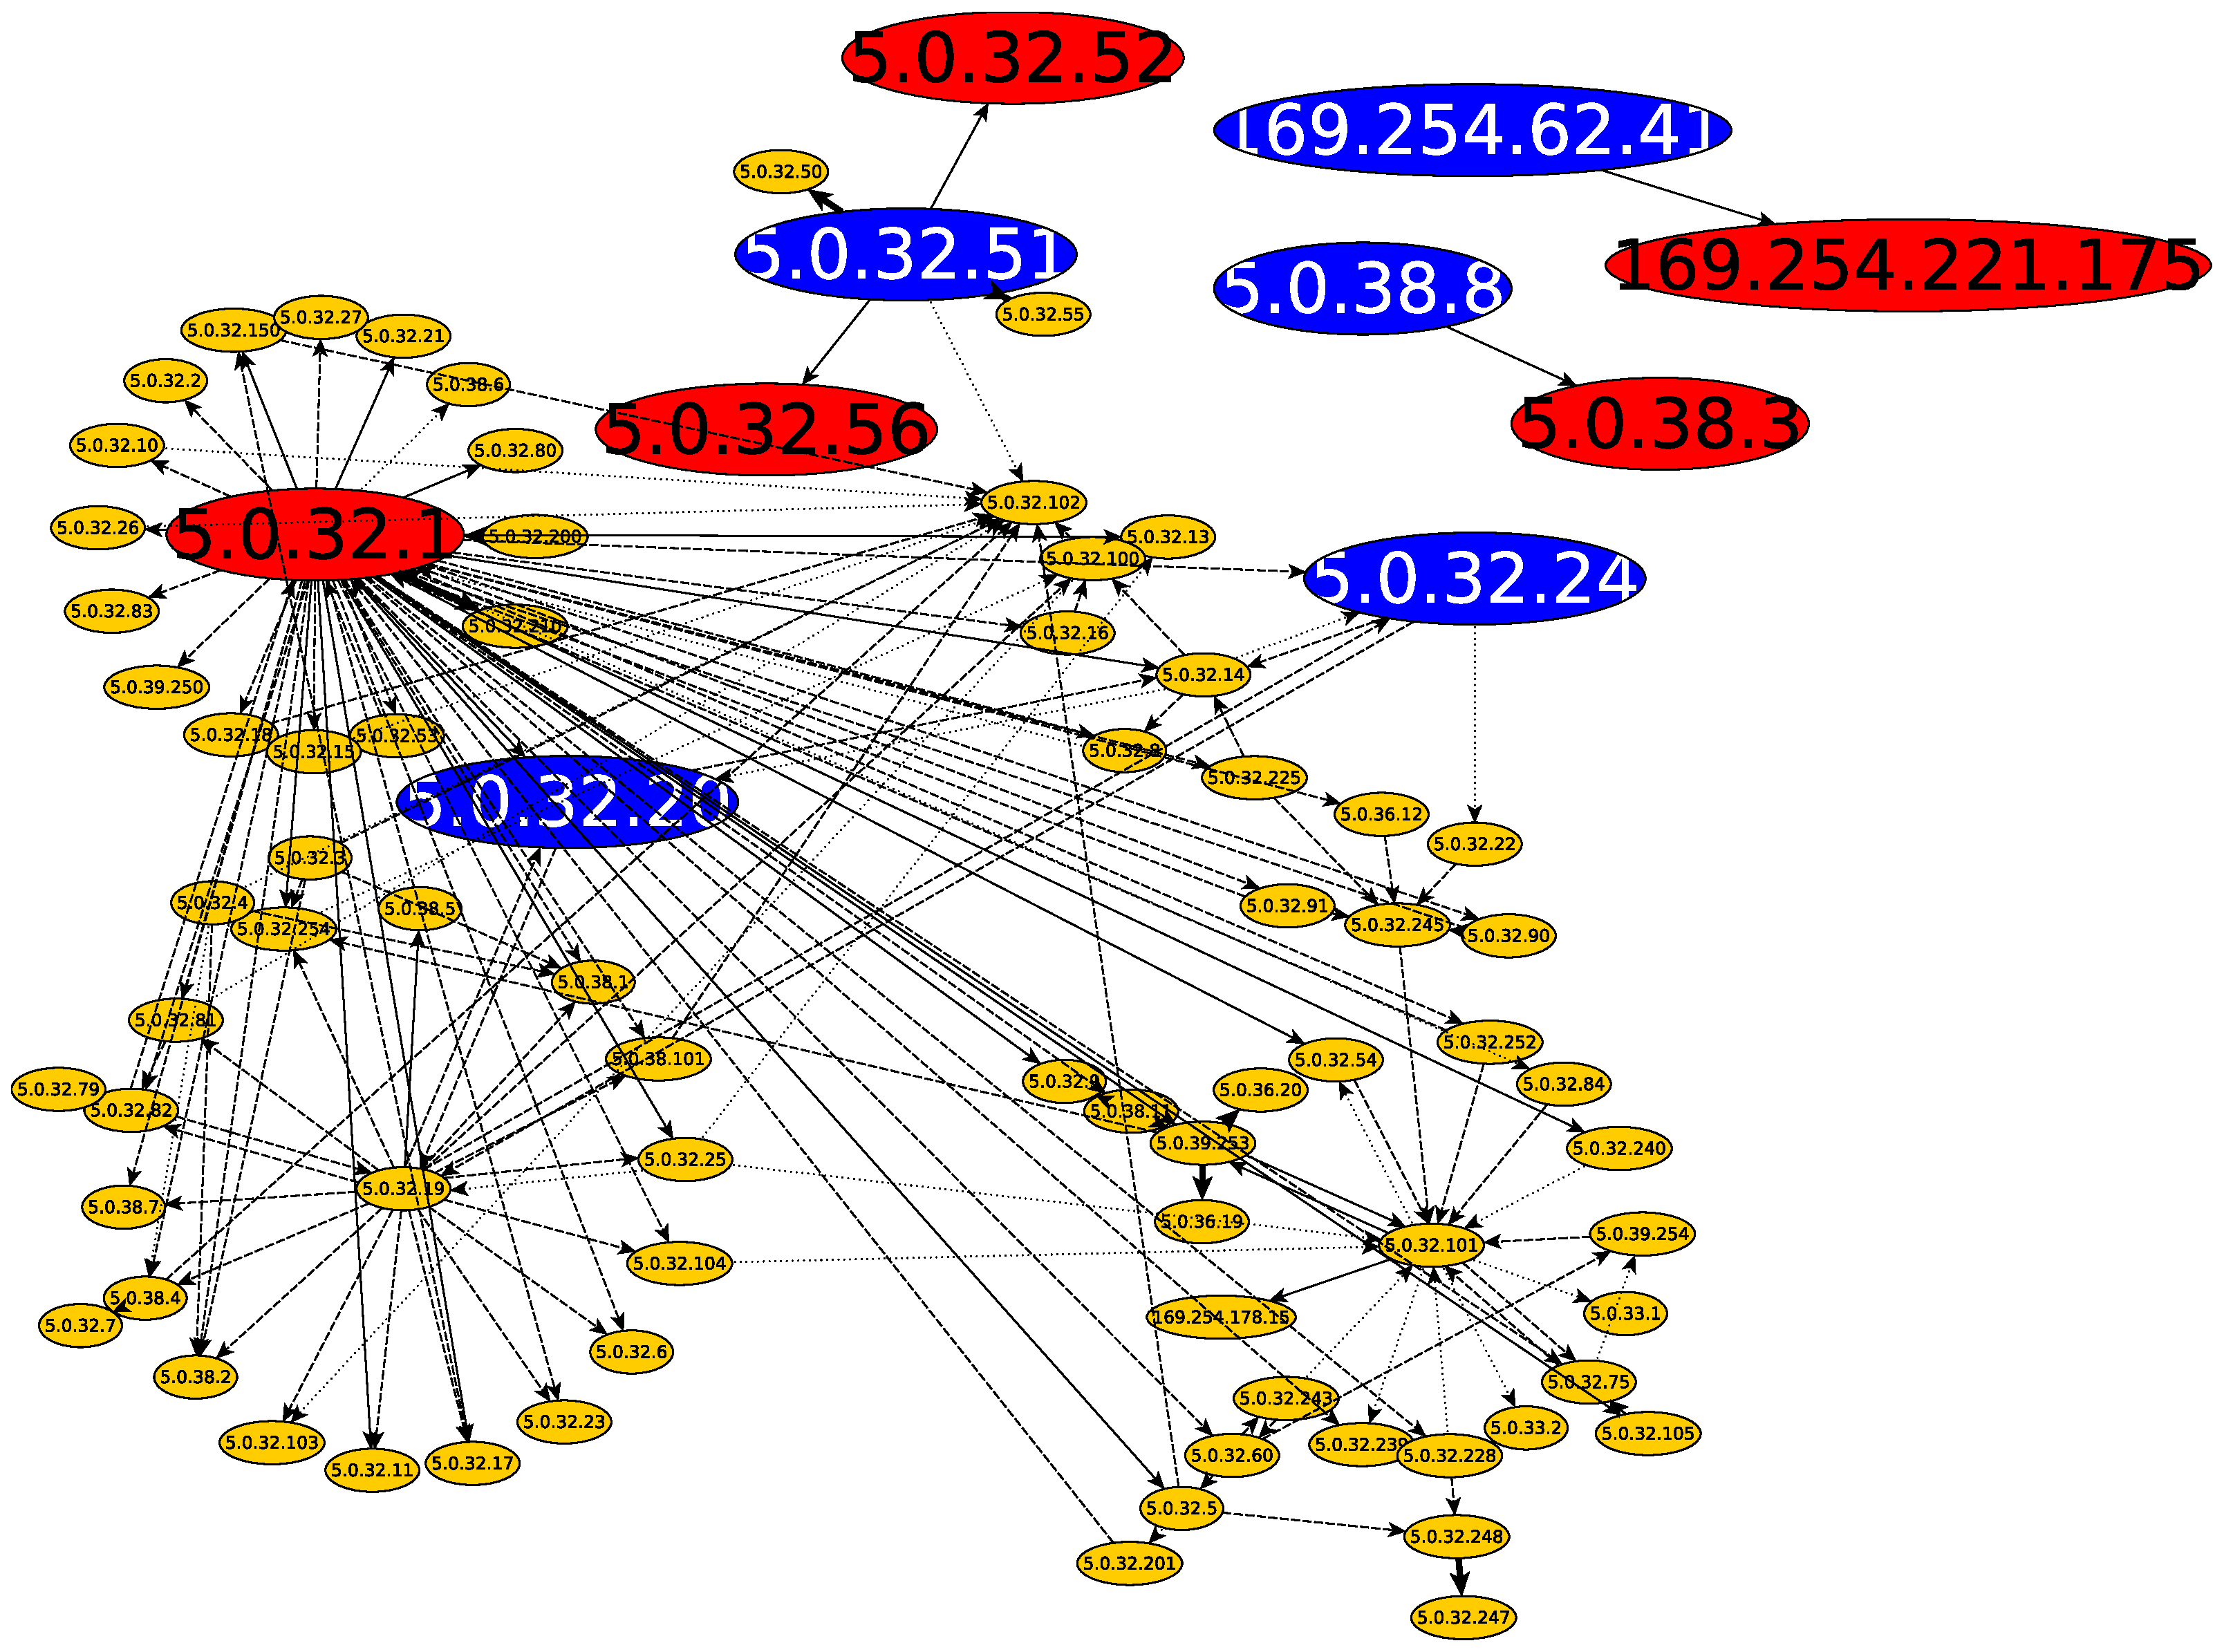
\includegraphics[width=\textwidth]{img/graph/escenario_1/vlan20/vlan20_70toEnd}
    \caption{Grafo VLAN \nameref{itm:vlan20}}
    \label{fig:vlan20_grafo}
\end{figure*}

\par En la figura \ref{fig:vlan20_grafo} se pueden observar ciertas cosas esperables
como otras que no tanto.

\par En primer lugar, salvo los nodos inclu\'idos en los percentiles 90, no pareciese
haber pedidos de resoluci\'on de \textit{MAC}\footnote{Abuso de notaci\'on.} entre
los hosts con poca probabilidad. Como posibles excepciones a esto se pueden ver las
IPs \textit{5.0.32.101, 5.0.32.19 y 5.0.32.102}. Si bien hay algunas otras con menor
afluencia que estas tres, hay que mencionar que ya en estas direcciones que mencionamos,
los ejes est\'an representados con flechas punteadas (es decir, no hay un pedido realmente
consistente de la \textit{MAC} de estos hosts).

\par Siguiendo con esta l\'inea de razonamiento, podemos ver que los ejes que denotan
"conexiones" consistentes entre servidores son pocos (lo cual es coherente con la
informaci\'on analizada hasta aqu\'i). Destacan por ah\'i algunas relaciones entre
la IP \textit{5.0.32.1}, claramente consultada por casi todos los nodos de la red (%
lo cual nos lleva a intu\'ir que este es un nodo importante de la red, ya que casi
todos en alg\'un momento durante la semana requieren poder conectarse a \'el) y 
los pedidos constantes de la \textit{5.0.32.51} para las direcciones \textit{5.0.32.56,
5.0.32.52, 5.0.32.50 y 5.0.32.55}\footnote{Estas \'ultimas dos ni siquiera forman
parte de uno de los percentiles 90}. Claramente aqu\'i, si consideramos que la
\textit{5.0.32.1} es posiblemente el \textit{gateway} de la red, nos encontramos
con 4 interfases de red que trabajan constantemente codo a codo (lo cual tambi\'en
explicar\'ia lo cercano de sus direcciones, aunque esto es simplemente algo que
se suele hacer en los \'ambitos de administraci\'on de servidores\footnote{Y \'unicamente
cuando los servidores son reci\'en instalados y hay IPs libres en la red.}).

\par Notoriamente, un resultado que no esper\'abamos encontrar es ver que parece
ser la \textit{5.0.32.1} el gateway de la red en lugar de la \textit{5.0.38.3} o la
\textit{5.0.38.8}, que son las direcciones con mayor probabilidad en ambas fuentes de informaci\'on.
Esto sorprende, pero como se ha dicho anteriormente, estando en una red de servidores no se espera
que estos deban de comunicarse con otras redes tan seguido como por ah\'i lo hacen
las terminales de otras redes (principalmeente porque los servidores se comunican
entre s\'i para la gran parte de sus tareas\footnote{Los servidores una vez instalados
no se actualizan jam\'as. \textit{If ain't broken, don't fix it}. Manual b\'asico
del administrador de servidores.}).

\par Prosiguiendo, se nota que el tr\'afico entre la \textit{5.0.38.8} hacia
la \textit{5.0.38.3} es constante, ya que esta \'ultima tiene la probabilidad
m\'as alta de la fuente de destino y la primera la tiene en la fuente de origen. Claramente
estas dos terminales deben estar proveyendo alg\'un tipo de servicio, o utilizando
una el servicio de la otra, constantemente, ya que sus probabilidades son
notoriamente mayores que la del resto de las IPs.

\subsubsection*{\underline{VLAN \nameref{itm:vlan20}: Conclusiones}}\label{subsubsec:vlan20_conclusiones}


    \subsubsection{VLAN de~\nameref{itm:vlan40}}
\par Para continuar con el estudio de las fuentes de paquetes ARP en distintas redes,
propusimos \textit{sniffear} una red local no tan convencional como lo son las
redes de computadoras ethernet o \textit{Wi-Fi}. Por ello trabajamos sobre una
red de telefon\'ia IP.

\par En esta redes los protocolos utilizados son los mismos que se vienen viendo
durante todo el trabajo. Aunque claramente, al ser los dispositivos tel\'efonos,
se espera ver un comportamiento distinto. En particular, este comportamiento
depender\'a de los dispositivos que componen a la red: los tel\'efonos IP.

\par Es de conocimiento en el \'area donde se ha realizado la tarea de recolecci\'on
datos, que estos dispositivos suelen tener comportamientos inesperados. De hecho,
en varios casos experimentados se observo como ciertas impresoras IP realizaban
env\'ios de paquetes \textit{broadcast} sin cesar, saturando el medio compartido
y, en la jerga informal, \textit{tirar abajo la red.}

\par Comenzamos como ven\'imos haciendo hasta ahora, con la entrop\'ia y los
datos generales de los datos obtenidos:

\begin{table}[!h]
\centering
  \begin{tabular}{c c}
    Fuente de Datos & Entrop\'ia \\
    \hline\hline
    Direcci\'on Origen & 0.0218949 \\
    Direcci\'on Destino & 5.20051 \\
    \hline\hline
    \#IPs de las Fuentes & 47\\
    \#Paquetes Capturados & 40034 \\
    \hline
    \end{tabular}
  \bigskip
  \caption{Entrop\'ia VLAN \nameref{itm:vlan40}}
  \label{tab:vlan40_entropia}
\end{table}

\par Ya de inmediato podemos ver que nos encontramos ante una LAN distinta. La entrop\'ia
de la fuente de origen es muy baja, lo cual nos da la pauta de que saber quienes son
los dispositivos que env\'ian paquetes ARP no deber\'ia ser algo incierto, sino todo
lo contrario.

\par Esto es entendible debido a que se ve que nos encontramos ante una red "peque\~na",
al menos considerando los 2 casos anteriores.


\subsubsection*{\underline{VLAN \nameref{itm:vlan40}: Fuente Origen}}\label{subsubsec:vlan40_src}
\par Veamos entonces como son las probabilidades de estas direcciones.

\begin{figure}[!ht]
    \centering
    \includegraphics[width=0.5\textwidth]{escenario_1/vlan40/vlan40_src_bars_percentile90}
    \caption{Probabilidades VLAN \nameref{itm:vlan40} - Fuente Origen}
    \label{fig:vlan40_src_prob_per90}
\end{figure}

\par Como se puede observar en la figura \ref{fig:vlan40_src_prob_per90}, ni siquiera
es necesario trabajar con el percentil 90. Hay tan pocas IPs, y -aparentemente- los
tel\'efonos no indundan la VLAN con paquetes de ARP. Esto podr\'ia deberse a muchos
distintos factores, como la configuraci\'on de estos y el software que utilizan%
\footnote{Es porbable que muchos tel\'efonos no requieran de enviar paquetes ARP ya
que por ah\'i memorizan la \textit{MAC} de la \textit{PBX} en caso de estar esta
en su LAN.}.

\par En cualquier caso, conviene observar que ocurre con la fuente de destino.
De momento lo \'unico que podemos decir es que los tel\'efonos no parecen
env\'iar demasiados paquetes ARP en la red.


\subsubsection*{\underline{VLAN \nameref{itm:vlan40}: Fuente Destino}}\label{subsubsec:vlan40_dst}

\begin{figure}[!ht]
    \centering
    \includegraphics[width=0.5\textwidth]{escenario_1/vlan40/vlan40_dst_bars_percentile90}
    \caption{Probabilidades VLAN \nameref{itm:vlan40} - Fuente Destino}
    \label{fig:vlan40_dst_prob_per90}
\end{figure}

\par Nuevamente nos encontramos con un caso impensado\footnote{Para el estudiante al menos}
en un principio. Se puede observar en la figura \ref{fig:vlan40_dst_prob_per90} que al
contrario de lo que ocurre  en la fuente de origen, en la red de telefon\'ia IP los dispositivos
tienen una distribuci\'on de la probabilidad aproximadamente equiprobable. Es decir, cada
tel\'efono, en su mayor\'ia, tiene la misma probabilidad que el resto de aparecer como
un mensaje devuelto por la fuente de informaci\'on que se est\'a estudiando.

\par Esto puede ser observado no solamente por las barras de probabilidad, sino por el
crecimiento lineal del percentil90, que no sindica que las probabilidades de cada
IP est\'an aportando aproximadamente lo mismo al percentil.

\par Es esperable ver entonces que la concentraci\'on de la probabilidad deber\'ia ser
un n\'umero que se acerque a 1 (al menos, que se acerque mucho m\'as que los casos
hasta ahora estudiados). Esto se debe a que vemos que el percentil 90 se
alcanza casi teniendo en cuenta las probabilidades de todas las IPs.

\begin{table}[!h]
\centering
  \begin{tabular}{c c c c}
    Fuente& 
    Entrop\'ia & \begin{tabular}{@{}c@{}}Concentraci\'on \\ Percentil 90\end{tabular} 
    & \begin{tabular}{@{}c@{}}Concentraci\'on \\ Percentil 80\end{tabular}\\
    \hline\hline
    Origen & 0.0218949 & 0.0021\% & 0.0021\%\\
    Destino & 5.20051 & 0.681\% & 0.553\%\\
    \hline\hline
    \end{tabular}
  \bigskip
  \caption{Concentraci\'on VLAN \nameref{itm:vlan10}}
  \label{tab:vlan40_concentracion}
\end{table}

\par Efectivamente, lo que se ven\'ia reflejando ahora tambi\'en se demuestra con los
valores del cuadro \ref{tab:vlan40_concentracion}. Vemos como la entrop\'ia de la fuente
de origen es muy baja, debido a que casi toda la probabilidad de la fuente se concentra
en una \'unica direcci\'on IP (ver figura \ref{fig:vlan40_src_prob_per90}), teniendo
al mismo tiempo una concentraci\'on muy baja del percentil 90 (al fin y al cabo, es
s\'olo una IP la que acumula todo).

\par Por el otro lado, vemos que como fuente de destino, nos encontramos con una concentraci\'on
del percentil m\'as alta que en casos anteriores. El hecho de que la probabilidad
sea casi equiprobable entre todos los s\'imbolos de la fuente nos da una entrop\'ia
relativamente alta para la cantidad de IPs que se tienen en la fuente (47). Esto se
debe a que al ser equiprobable\footnote{Apr\'oximadamente} el espacio de s\'imbolos
de la fuente, hay una gran incertidumbre que no nos permite asegurar con una buena
base estad\'istica sobre quienes son los datos m\'as probables que nos dar\'a la
fuente.

\subsubsection*{\underline{VLAN \nameref{itm:vlan40}: Ambas Fuentes}}\label{subsubsec:vlan40_src_dst}
\par Dado que estamos en una red chica y, aparentemente poco densa, sumado a la
probabilidad concentrada de la fuente de origen y la distribu\'ida de la fuente destino,
nos da a entender que nos encontraremos con una topolog\'ia donde todos se comunican
con la IP \textit{5.0.48.1}\footnote{\nameref{fig:vlan40_src_prob_per90}.}.

\begin{figure}[ht]
    \centering
    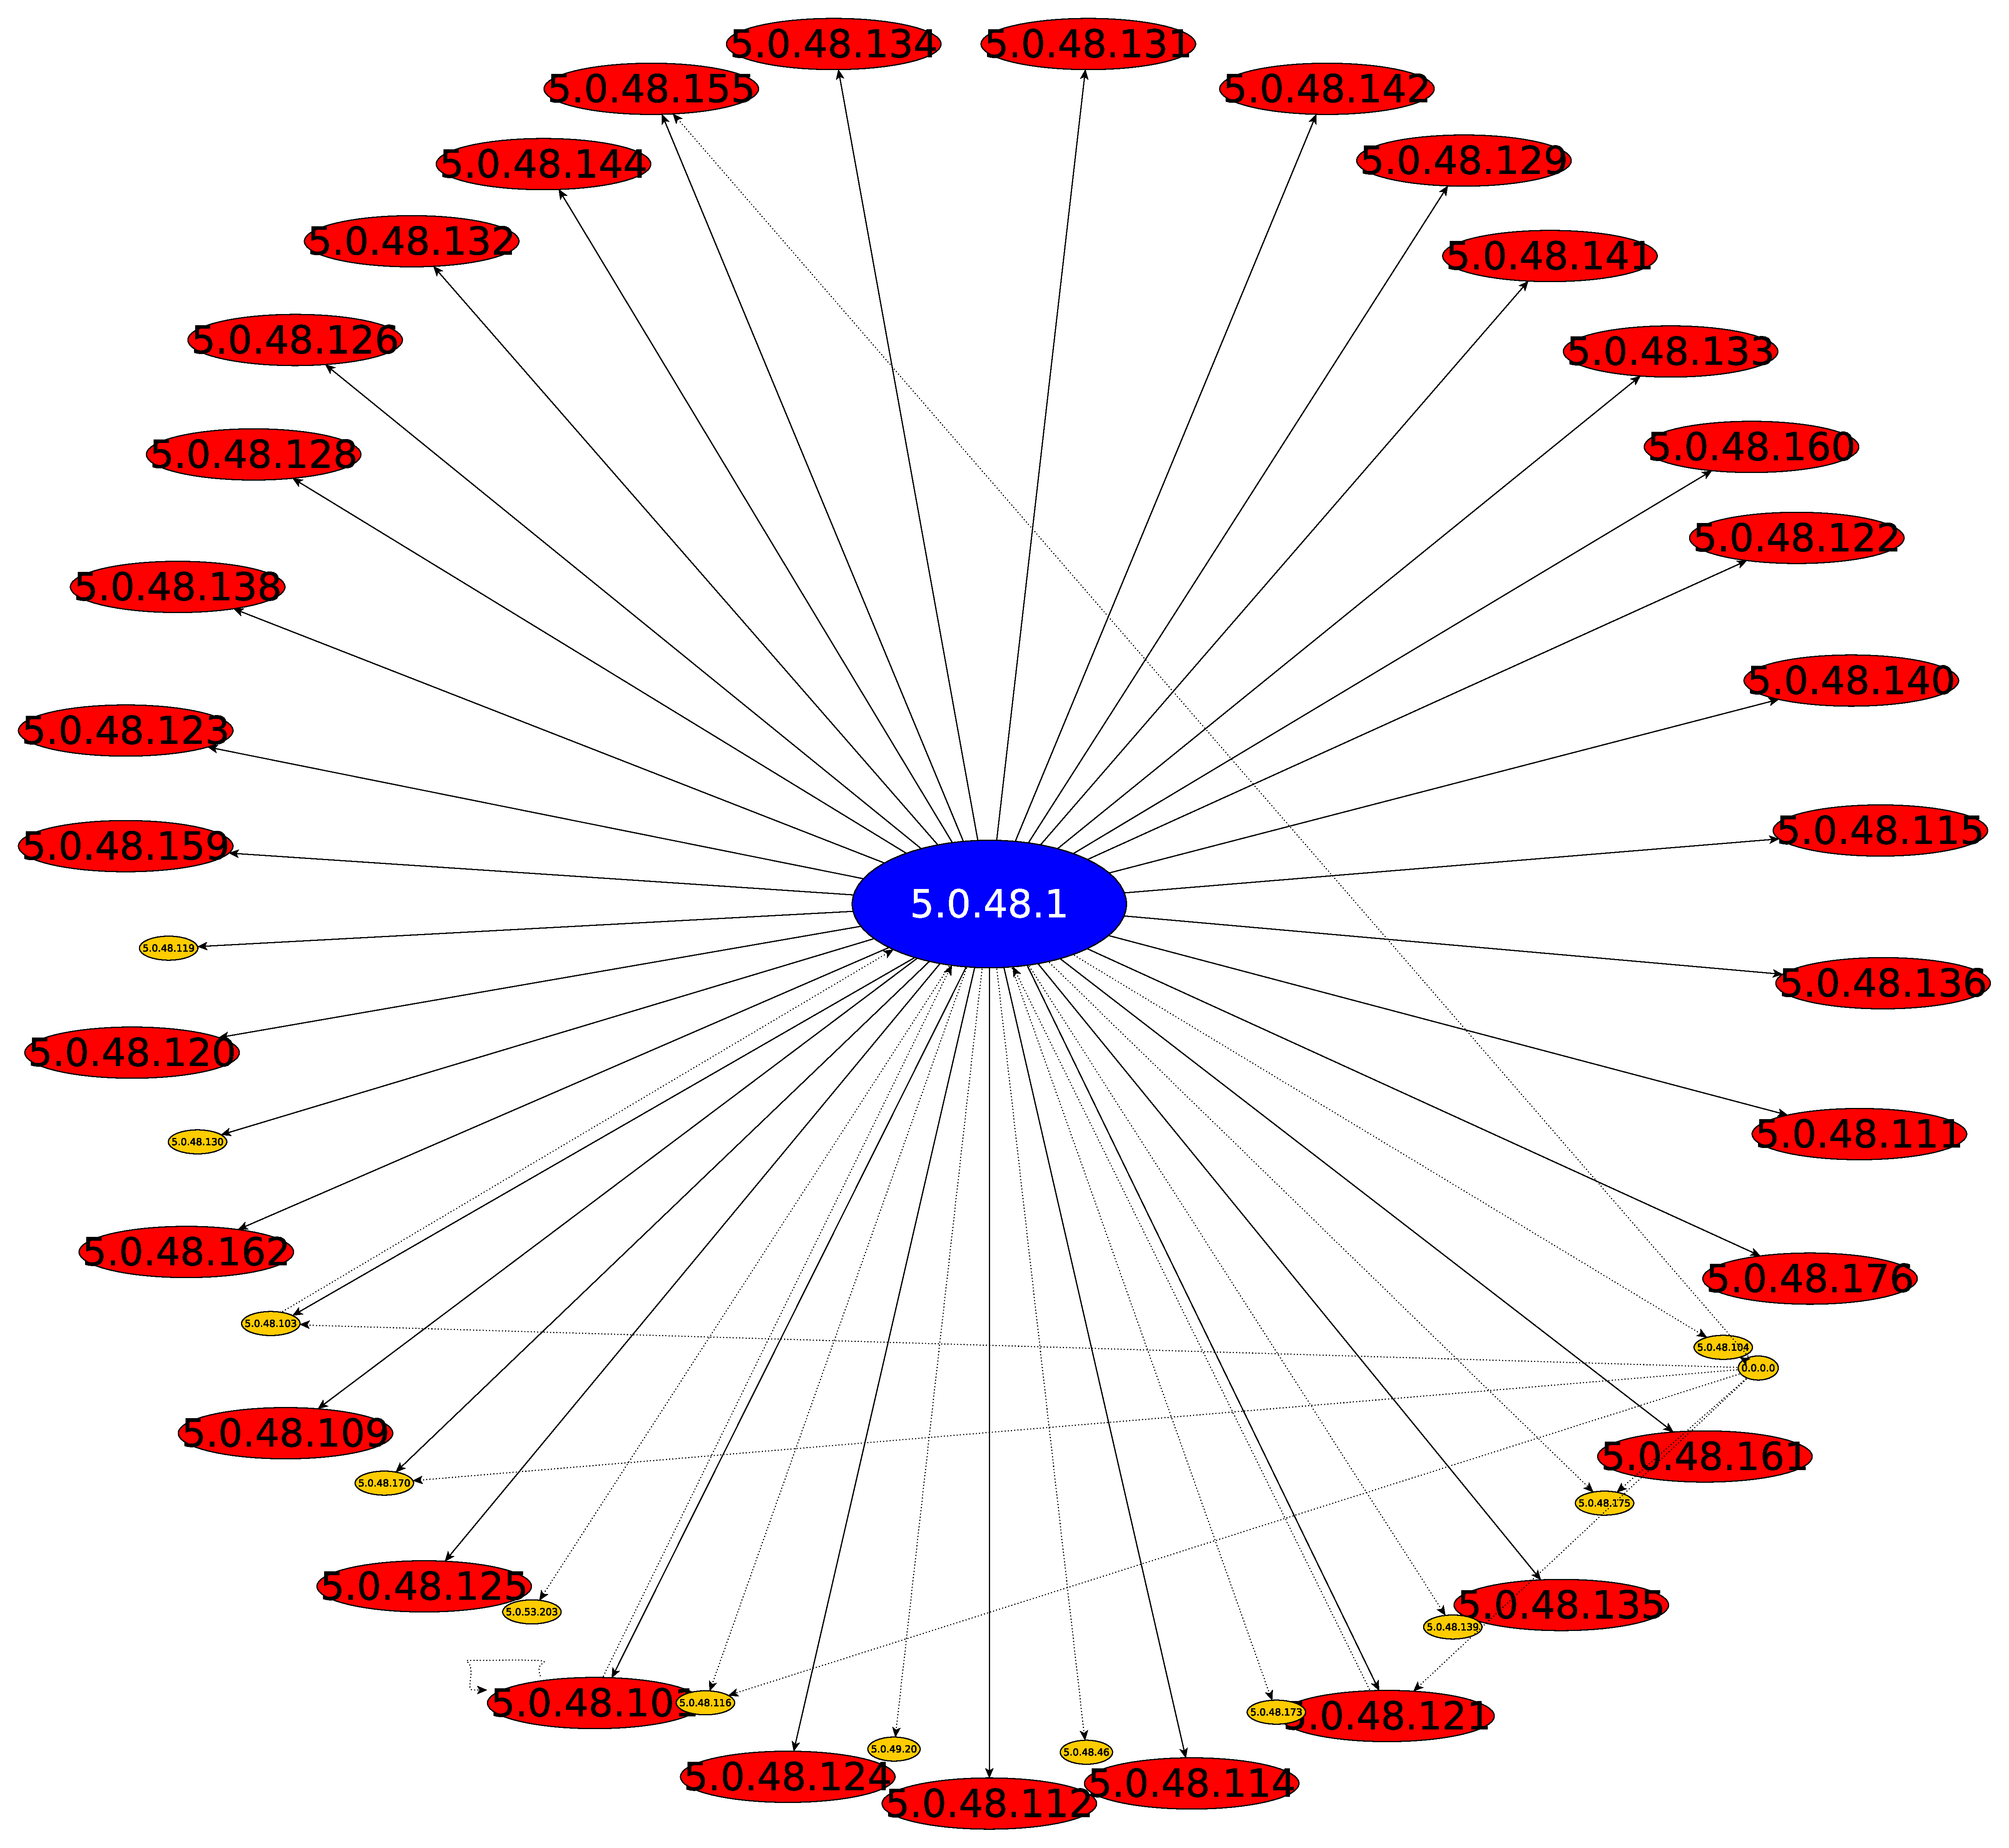
\includegraphics[width=0.5\textwidth]{img/graph/escenario_1/vlan40/vlan40}
    \caption{Grafo VLAN \nameref{itm:vlan40}}
    \label{fig:vlan40_grafo}
\end{figure}

\par Efectivamente se puede observar en el grafo que la red de tel\'efonia
IP parece trabajar con una topolog\'ia centralizada, al menos para cada vez
que deben resolver una \textit{MAC}, presumiblemente para realizar alguna
tarea que requiera de la utilizaci\'on de la red\footnote{Eso o la
telefon\'ia IP se utiliza muy poco en el datacenter.}.

\par As\'i pues, queda claro en la figura \ref{fig:vlan40_grafo} que nos encontramos
con un nodo principal que seguramente es la \textit{PBX} o servidor del
servicio de tel\'efon\'ia m\'ovil.


\subsubsection*{\underline{VLAN \nameref{itm:vlan40}: Conclusiones}}\label{subsubsec:vlan40_conclusiones}
\par Aqu\'i nos encontramos con una red que claramente se comporta distinta que el resto.
De la informaci\'on recolectada y los an\'alisis realizados, se pudo ver que
hay muy poco tr\'afico y por ende los valores de entrop\'ia y la cantidad
de IPs de la LAN nos permiten anticipar el comportamiento de la LAN sin
conocer detalles t\'ecnicos sobre la infraestructura o el software que 
utilizan los tel\'efonos.


    \subsubsection{VLAN de~\nameref{itm:vlan1}}
\par Para finalizar con las tareas requeridas por este trabajo en cuanto
a el \nameref{sec:escenario1}, se pasa a analizar la \textit{dataset} m\'as
grande de todos los capturados.

\par Como ya se describi\'o, la VLAN de \nameref{itm:vlan1} consta de una
gran variedad de diferentes dispositivos que cubren una extensa zona geogr\'afica.

\par Esta red originalmente era utilizada para tener una \'unica red para
todos los servicios y usuarios del organismo que n\'uclea al \textit{datacenter}.

\par As\'i pues, esperamos encontrarnos con una red con alta cantidad de 
paquetes ARP inundando el dominio de colisi\'on, y con una enorme cantidad
de distintas direcciones IP\footnote{La red en cuesti\'on es una red
clase \textit{A}}.

\par Siguiendo con el orden establecido en los casos anteriores, comenzaremos
presentando los resultados de los c\'alculos de entrop\'ia de ambas fuentes,
m\'as las caracter\'isticas del \textit{dataset}:

\begin{table}[!h]
\centering
  \begin{tabular}{c c}
    Fuente de Datos & Entrop\'ia \\
    \hline\hline
    Direcci\'on Origen & 5.8538 \\
    Direcci\'on Destino &  9.45154 \\
    \hline\hline
    \#IPs de las Fuentes & 50\,733 \\
    \#Paquetes Capturados & 11\,265\,364 \\
    \hline
    \end{tabular}
  \bigskip
  \caption{Entrop\'ia VLAN \nameref{itm:vlan1}}
  \label{tab:vlan1_entropia}
\end{table}

\par Ni bien presentado estos datos, llama la atenci\'on que de est\'as fuentes
de informaci\'on, que intu\'imos por el conocimiento de la red que tenemos, que
ser\'a m\'as ca\'otica (y por lo tanto ser\'ia esperable encontrarnos con una
alta entrop\'ia), nos da valores similiares a las fuentes de informaci\'on
presentadas en las secciones anteriores\footnote{Aunque claramente estos valores
son superiores a los ya expuestos, se esperaba una diferencia a\'un m\'as amplia.}


\subsubsection*{\underline{VLAN \nameref{itm:vlan1}: Fuente Origen}}\label{subsubsec:vlan1_src}
\par Se incluye a continuaci\'on las probabilidades por s\'imbolo de la fuente de direcci\'on
origne en la figura \ref{fig:vlan1_src_prob_per90}

\begin{figure}[!ht]
    \centering
    \includegraphics[width=0.5\textwidth]{escenario_1/vlan1/vlan1_src_bars_percentile90}
    \caption{Probabilidades VLAN \nameref{itm:vlan1} - Fuente Origen}
    \label{fig:vlan1_src_prob_per90}
\end{figure}

\par Al igual que en los casos anteriores donde tuvimos una entrop\'ia alta, se observa
en el gr\'afico que el percentil 90 se encuentra contenido en un porcentaje muy peque\~no
del total de s\'imbolos/IPs que provee la fuente de informaci\'on. Si bien, pareciese
que 260 IPs es un n\'umero grande si tenemos en cuenta las cantidades que venimos
analizando, no hay que perder de vista que en esta fuente obtuvimos un total de
50\,733 s\'imbolos distintos (n\'umero que supera con creces los hasta ahora vistos).

\par Si nos concentramos en las primeras 25 IPs, observamos que el percentil de la probabilidad
es el 70, el cu\'al nos muestra a\'un m\'as claramente la concentraci\'on de la informaci\'on
en las IPs con mayor probabilidad. Con 260 IPs se tiene un 90\% de la probabilidad mientras
que con 70 (menos de un tercio) se acumula un 70\%.

\begin{figure}[!ht]
    \centering
    \includegraphics[width=0.5\textwidth]{escenario_1/vlan1/vlan1_src_probabilities_with_labels}
    \caption{IPs VLAN \nameref{itm:vlan1} - Fuente Origen}
    \label{fig:vlan1_src_prob_ips}
\end{figure}

\par Ya podemos entonces ir viendo que tendremos unos serios candidatos a nodos
importantes de la red a:

\begin{itemize}
    \item \textit{5.0.0.18}
    \item \textit{5.0.0.20}
    \item \textit{5.0.0.19}
    \item \textit{10.1.254.5}
    \item \textit{10.13.100.15}
    \item \textit{5.0.96.37}
\end{itemize}


\subsubsection*{\underline{VLAN \nameref{itm:vlan1}: Fuente Destino}}\label{subsubsec:vlan1_dst}
\par Sabiendo ya que para la fuente de destino tenemos una entrop\'ia de casi el
doble de la obtenida para la fuente de origen, es normal imaginar que nos
encontraremos cun un percentil 90 menos contenido. Si las matem\'aticas coinciden,
deber\'ia de ser de casi el doble de IPs.

\begin{figure}[!ht]
    \centering
    \includegraphics[width=0.5\textwidth]{escenario_1/vlan1/vlan1_dst_bars_percentile90}
    \caption{Probabilidades VLAN \nameref{itm:vlan1} - Fuente Destino}
    \label{fig:vlan1_dst_prob_per90}
\end{figure}

\par Efectivamente queda expl\'icito que se necesitan m\'as del doble de las IPs de mayor
probabilidad muestral para poder alcanzar el percentil 90. A\'un as\'i, con 850 IPs
segu\'imos muy lejos del total de s\'imbolos obtenidos de la fuente. Es decir,
la acumulaci\'on de la alta probabilidad en un numero reducido de IPs (aunque nominalmente
grande) nos da cierta informaci\'on sobre el comportamiento de la red, ya que la mayor
parte de la informaci\'on que da la fuente es reducida estad\'isticamente a un set
limitado\footnote{850 IPs contra 50\,733 es una diferencia nada desestimable.}.


\begin{table}[!h]
\centering
  \begin{tabular}{c c c c}
    Fuente& 
    Entrop\'ia & \begin{tabular}{@{}c@{}}Concentraci\'on \\ Percentil 90\end{tabular} 
    & \begin{tabular}{@{}c@{}}Concentraci\'on \\ Percentil 80\end{tabular}\\
    \hline\hline
    Origen & 5.8538 & 0.0045\% & 0.0012\%\\
    Destino & 9.45154 & 0.017\% & 0.008\%\\
    \hline\hline
    \end{tabular}
  \bigskip
  \caption{Concentraci\'on VLAN \nameref{itm:vlan1}}
  \label{tab:vlan1_concentracion}
\end{table}

\par Concentr\'emonos ahora en identificar posibles IPs importantes dentro de la red.
Para ello se presenta el siguiente gr\'afico con las 25 IPs con mayor probabilidad
de la fuente destino:

\begin{figure}[!ht]
    \centering
    \includegraphics[width=0.5\textwidth]{escenario_1/vlan1/vlan1_dst_probabilities_with_labels}
    \caption{IPs VLAN \nameref{itm:vlan1} - Fuente Destino}
    \label{fig:vlan1_dst_prob_ips}
\end{figure}

\par Se puede observar aqu\'i que claramente los s\'imbolos que m\'as probabilidad muestral
acumulan son los primeros 15 de la figura \ref{fig:vlan1_dst_prob_ips}.


\subsubsection*{\underline{VLAN \nameref{itm:vlan1}: Ambas Fuentes}}\label{subsubsec:vlan1_src_dst}
\par A continuaci\'on se muestra un grafo con la informaci\'on tomada durante la semana de
captura de paquetes ARP. En el mismo, al igual que en casos anteriores, se
desestiman aquellos ejes que no tengan un peso superior a 1000 (es decir, que
no hayan sido env\'iados m\'as de 1000 veces con las mismas direcciones
origen y destino), ya que en el largo trayecto que se tomaron los datos
de la fuente de informaci\'on, dichos casos no aportan mucho a identificar
patrones constantes sobre el comportamiento de la red.

\par La figura \ref{fig:vlan1_grafo} nos muestra dicho grafo. Se ve que el mismo es muy grande
(como se esperaba) y deberemos analizarlo por partes para que se puedan sacar
conclusiones.

\par En un principio podemos observar que el grafo cuenta con 8 regiones bien delimitadas
a simple vista. Desde la componente no conexa que se ubica en la parte superior
derecha del grafo hasta las diferentes \textit{circunferencias} de nodos que parecen
tener un nodo importante, o al menos con muchos ejes, en el centro.

\par Curiosamente, estos nodos en el centro de estas \textit{circunferencias} suelen
tener ejes que los unan con los nodos que los rodean y ejes que los unen entre si. Pero,
si bien se ven algunas peticiones entre nodos centrales y nodos perif\'ericos de otras
circunferencias, esta no es la norma. Esto nos lleva ya a apuntar a que (sumado a los
colores de dichos nodos centrales), estos hosts representan o cumplen alguna funci\'on
destacable dentro de la red.

\begin{figure*}
    \centering
    \includegraphics[width=\textheight,angle=90]{img/graph/escenario_1/vlan1/vlan1_1000toEnd}
    \caption{Grafo VLAN \nameref{itm:vlan1}}
    \label{fig:vlan1_grafo}
\end{figure*}

\newpage
\par Comenzando a analizar la region disconexa, se puede ver detalladamente en la figura
~\ref{fig:vlan1_grafo_unconexed} que la mayor\'ia de las peticiones que ocurren son entre
pares de nodos (y siempre el mismo par ordenado). As\'i pues se ven ciertas conexiones
entre varios nodos hacia una misma direcci\'on, pero nunca en grandes cantidades y siempre
limitado a no m\'as de 5 direcciones origen. Esto parecer\'ia describir el comportamiento
que ocurre en ciertas oficinas de trabajo al compartir archivos por la red (o quiz\'as al
trabajar con los servicios de un servidor peque\~no).

\begin{figure}[!htb]
    \centering
    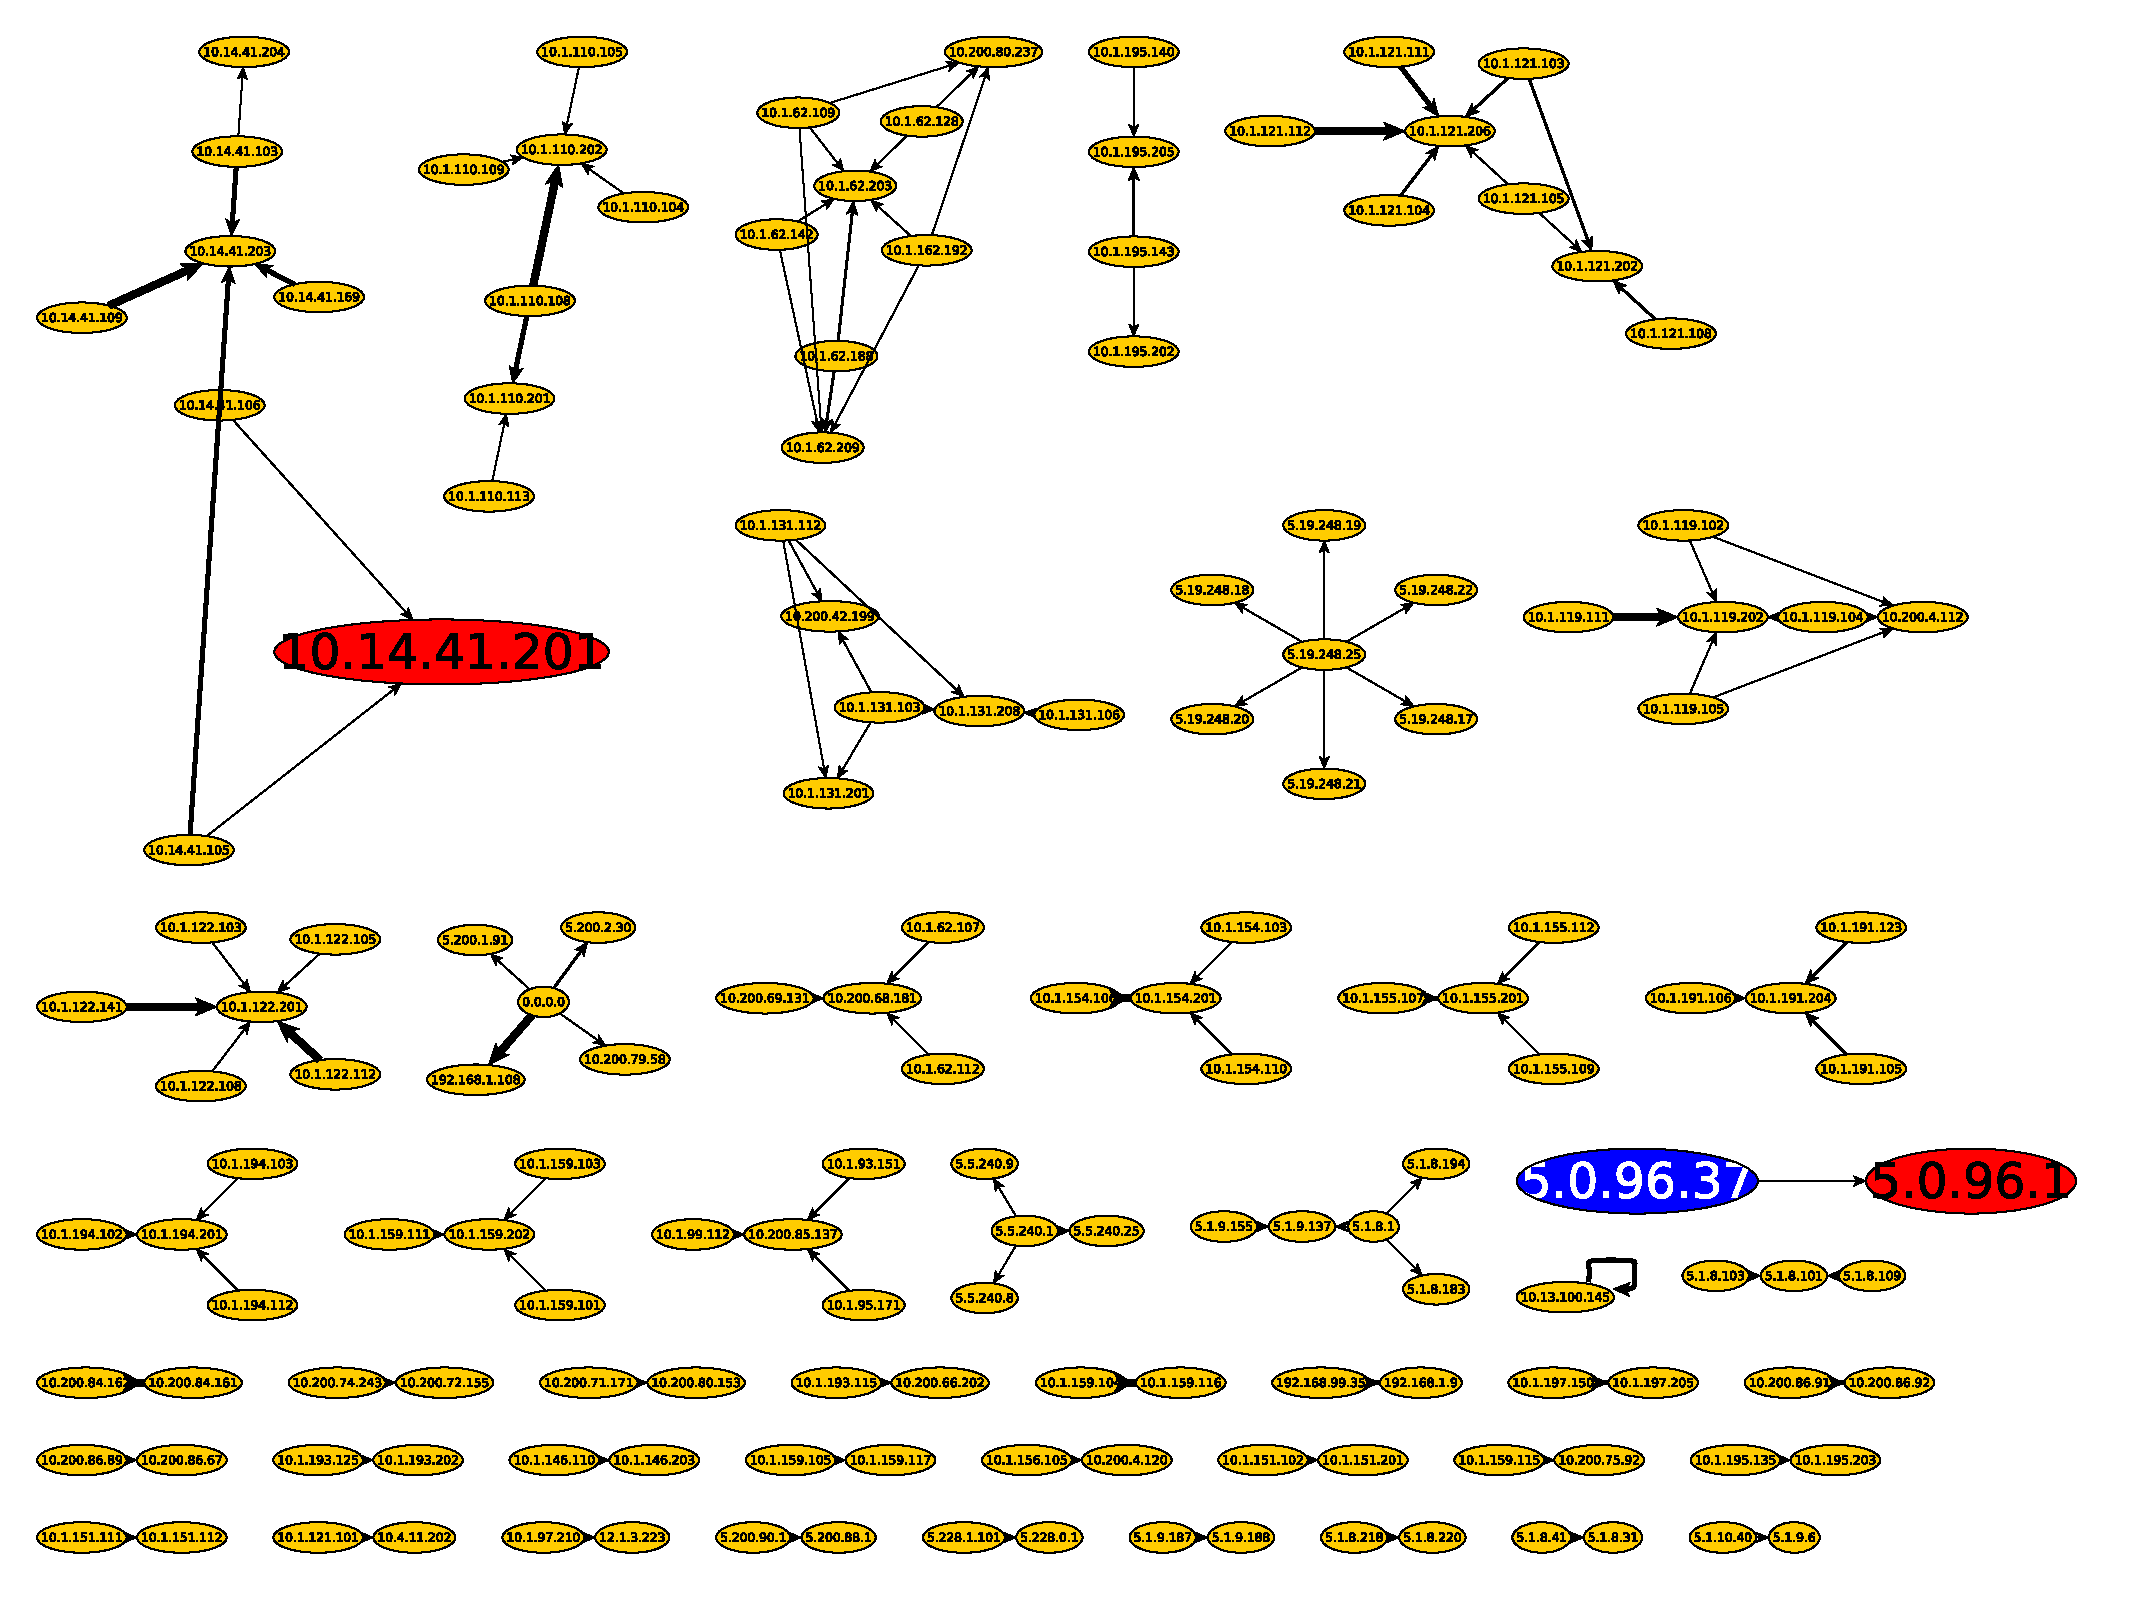
\includegraphics[width=0.5\textwidth]{img/graph/escenario_1/vlan1/vlan1_1000toEnd_unconexed}
    \caption{VLAN \nameref{itm:vlan1} - Componente Disconexo}
    \label{fig:vlan1_grafo_unconexed}
\end{figure}


\par Enfoc\'andonos sobre uno de los nodos ya se\~nalados en el inciso \ref{subsubsec:vlan1_src},
(figura \ref{fig:vlan1_grafo_10_0_0_19})
observamos que todos los paquetes constantes ARP tiene a la IP \textit{10.0.0.19} como direcci\'on
de origen. As\'i pues ser\'ia valido pensar que dicho host o se encuentra \textit{scanneando} la
red en busca siempre de las mismas IPs, o se trata de alg\'un servidor encargado de ofrecer
un servicio a un conjunto limitado de m\'aquinas de la red\footnote{NFS, Samba, DHCP, antivirus etc} o
quiz\'as de un equipo que se encuentra monitoreando a las otras direcciones.

\begin{figure}[!ht]
    \centering
    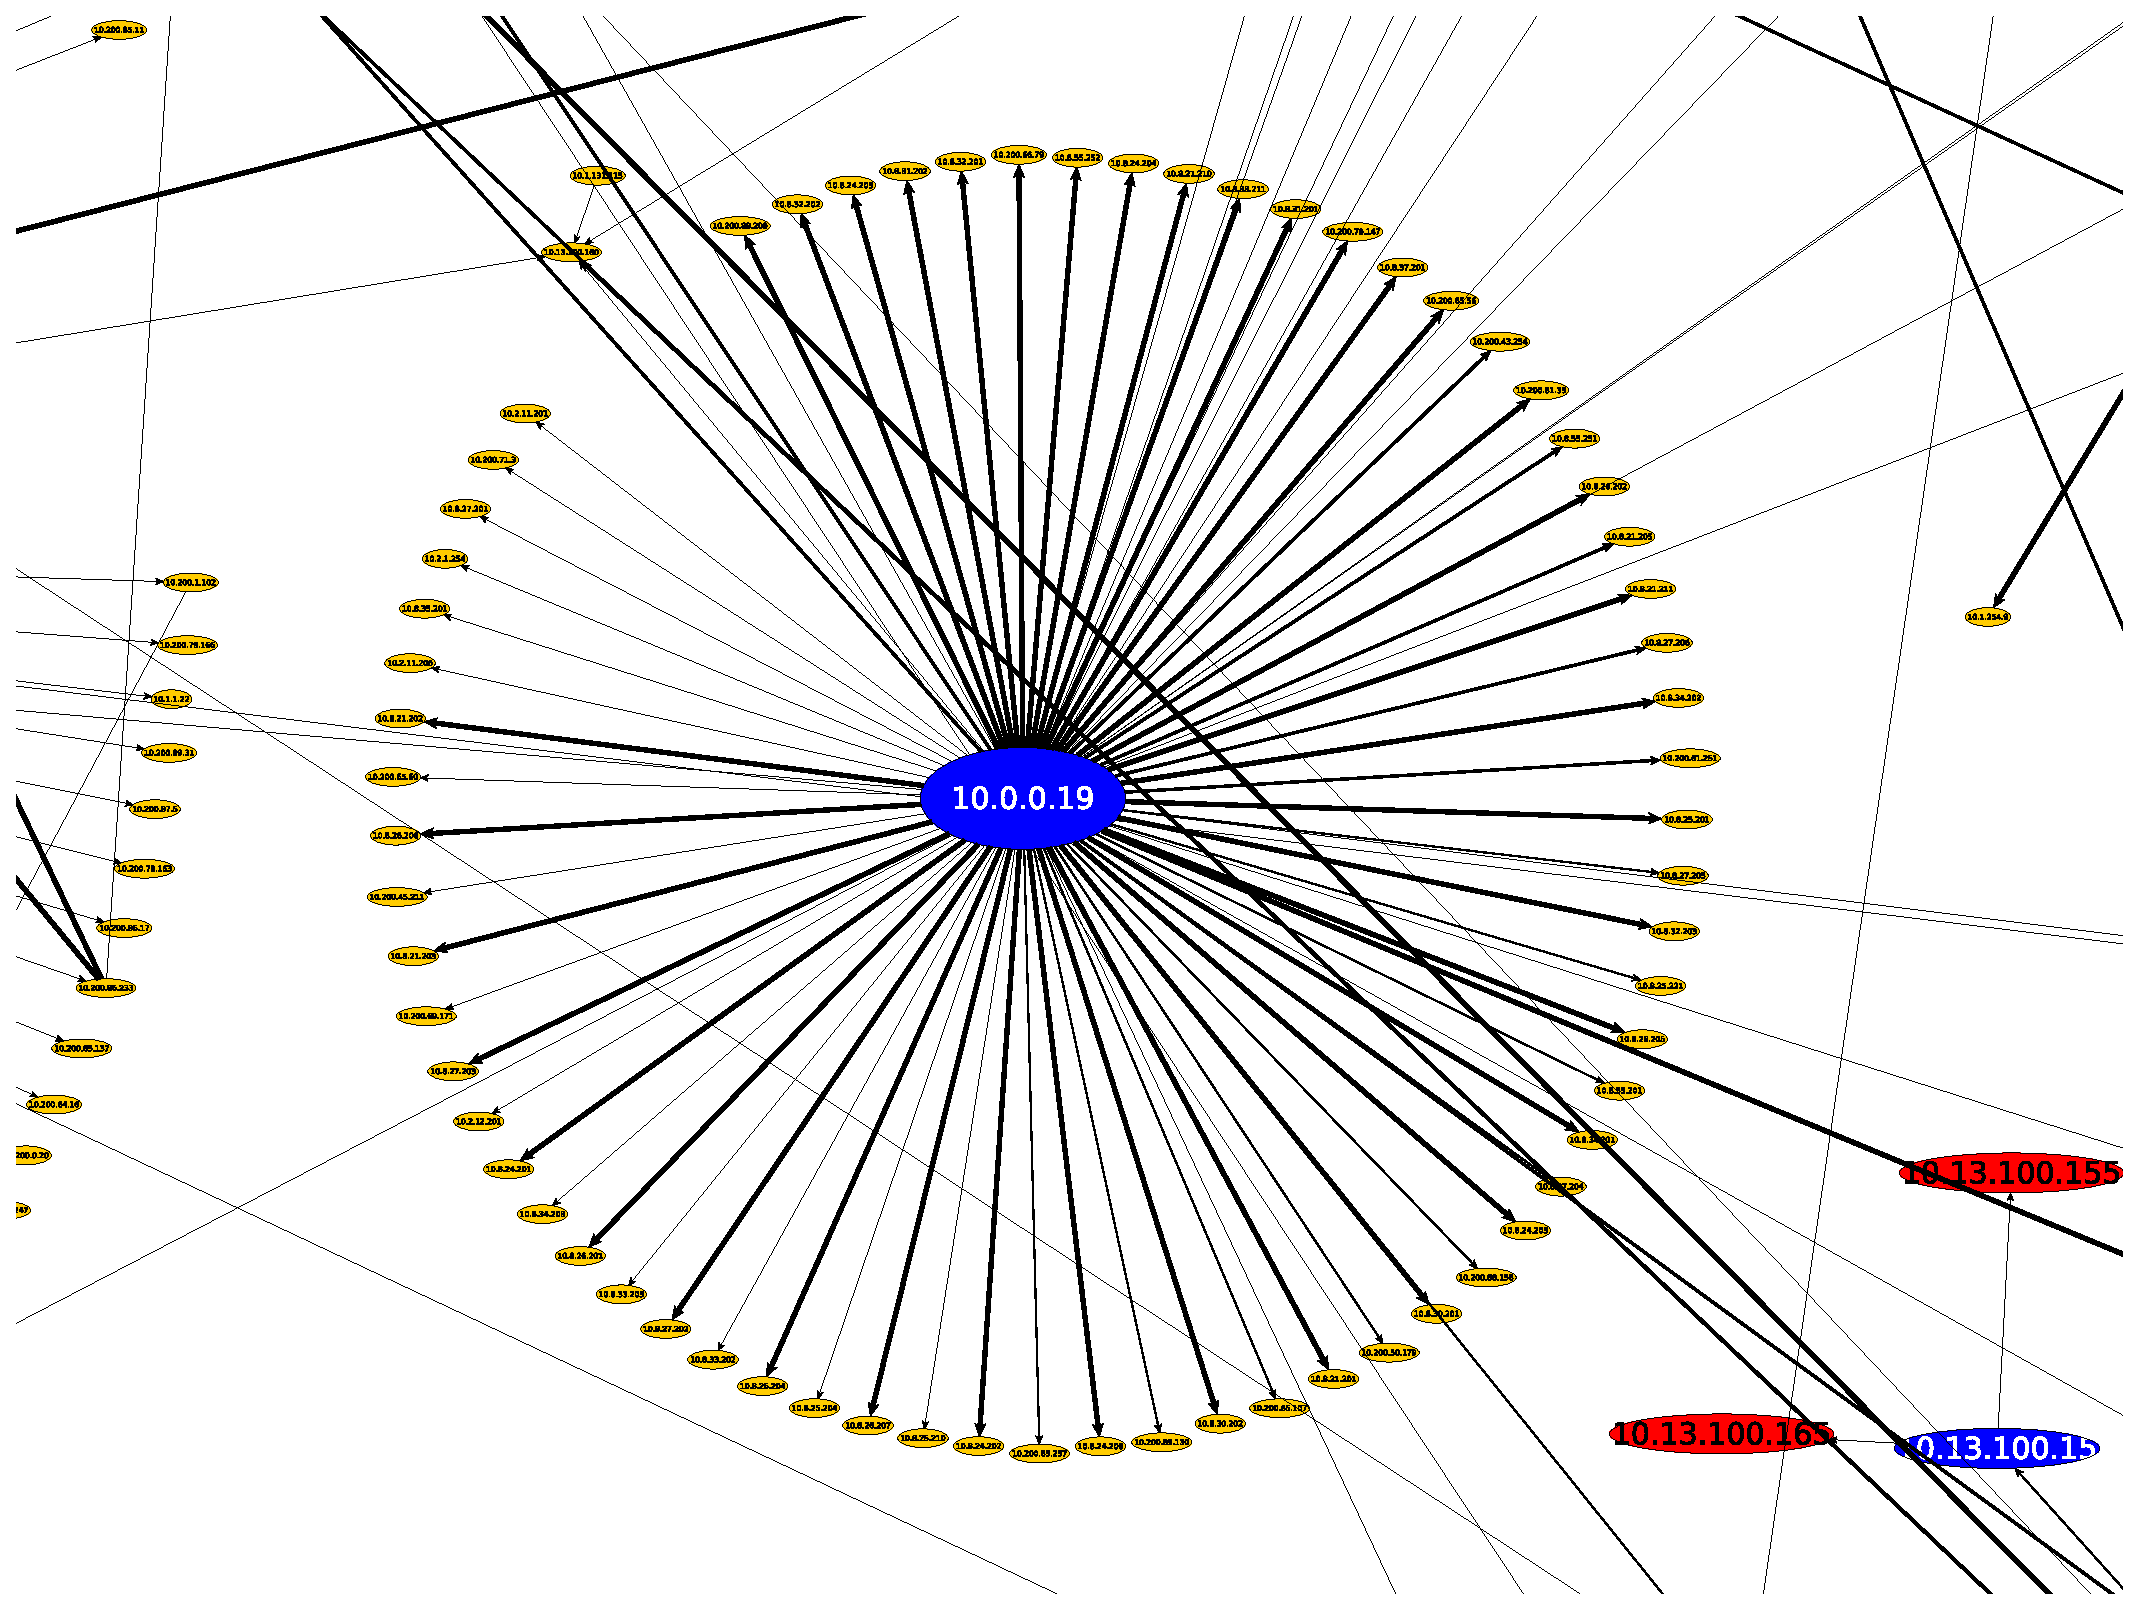
\includegraphics[width=0.5\textwidth]{img/graph/escenario_1/vlan1/vlan1_1000toEnd_10_0_0_19}
    \caption{VLAN \nameref{itm:vlan1} - 10.0.0.19}
    \label{fig:vlan1_grafo_10_0_0_19}
\end{figure}

\par Esto mismo aplica a las IPs \textit{10.0.0.18} y \textit{10.0.0.20}, tal como se puede ver
en las figuras \ref{fig:vlan1_grafo_10_0_0_18} y \ref{fig:vlan1_grafo_10_0_0_20}.

\begin{figure}[!ht]
    \centering
    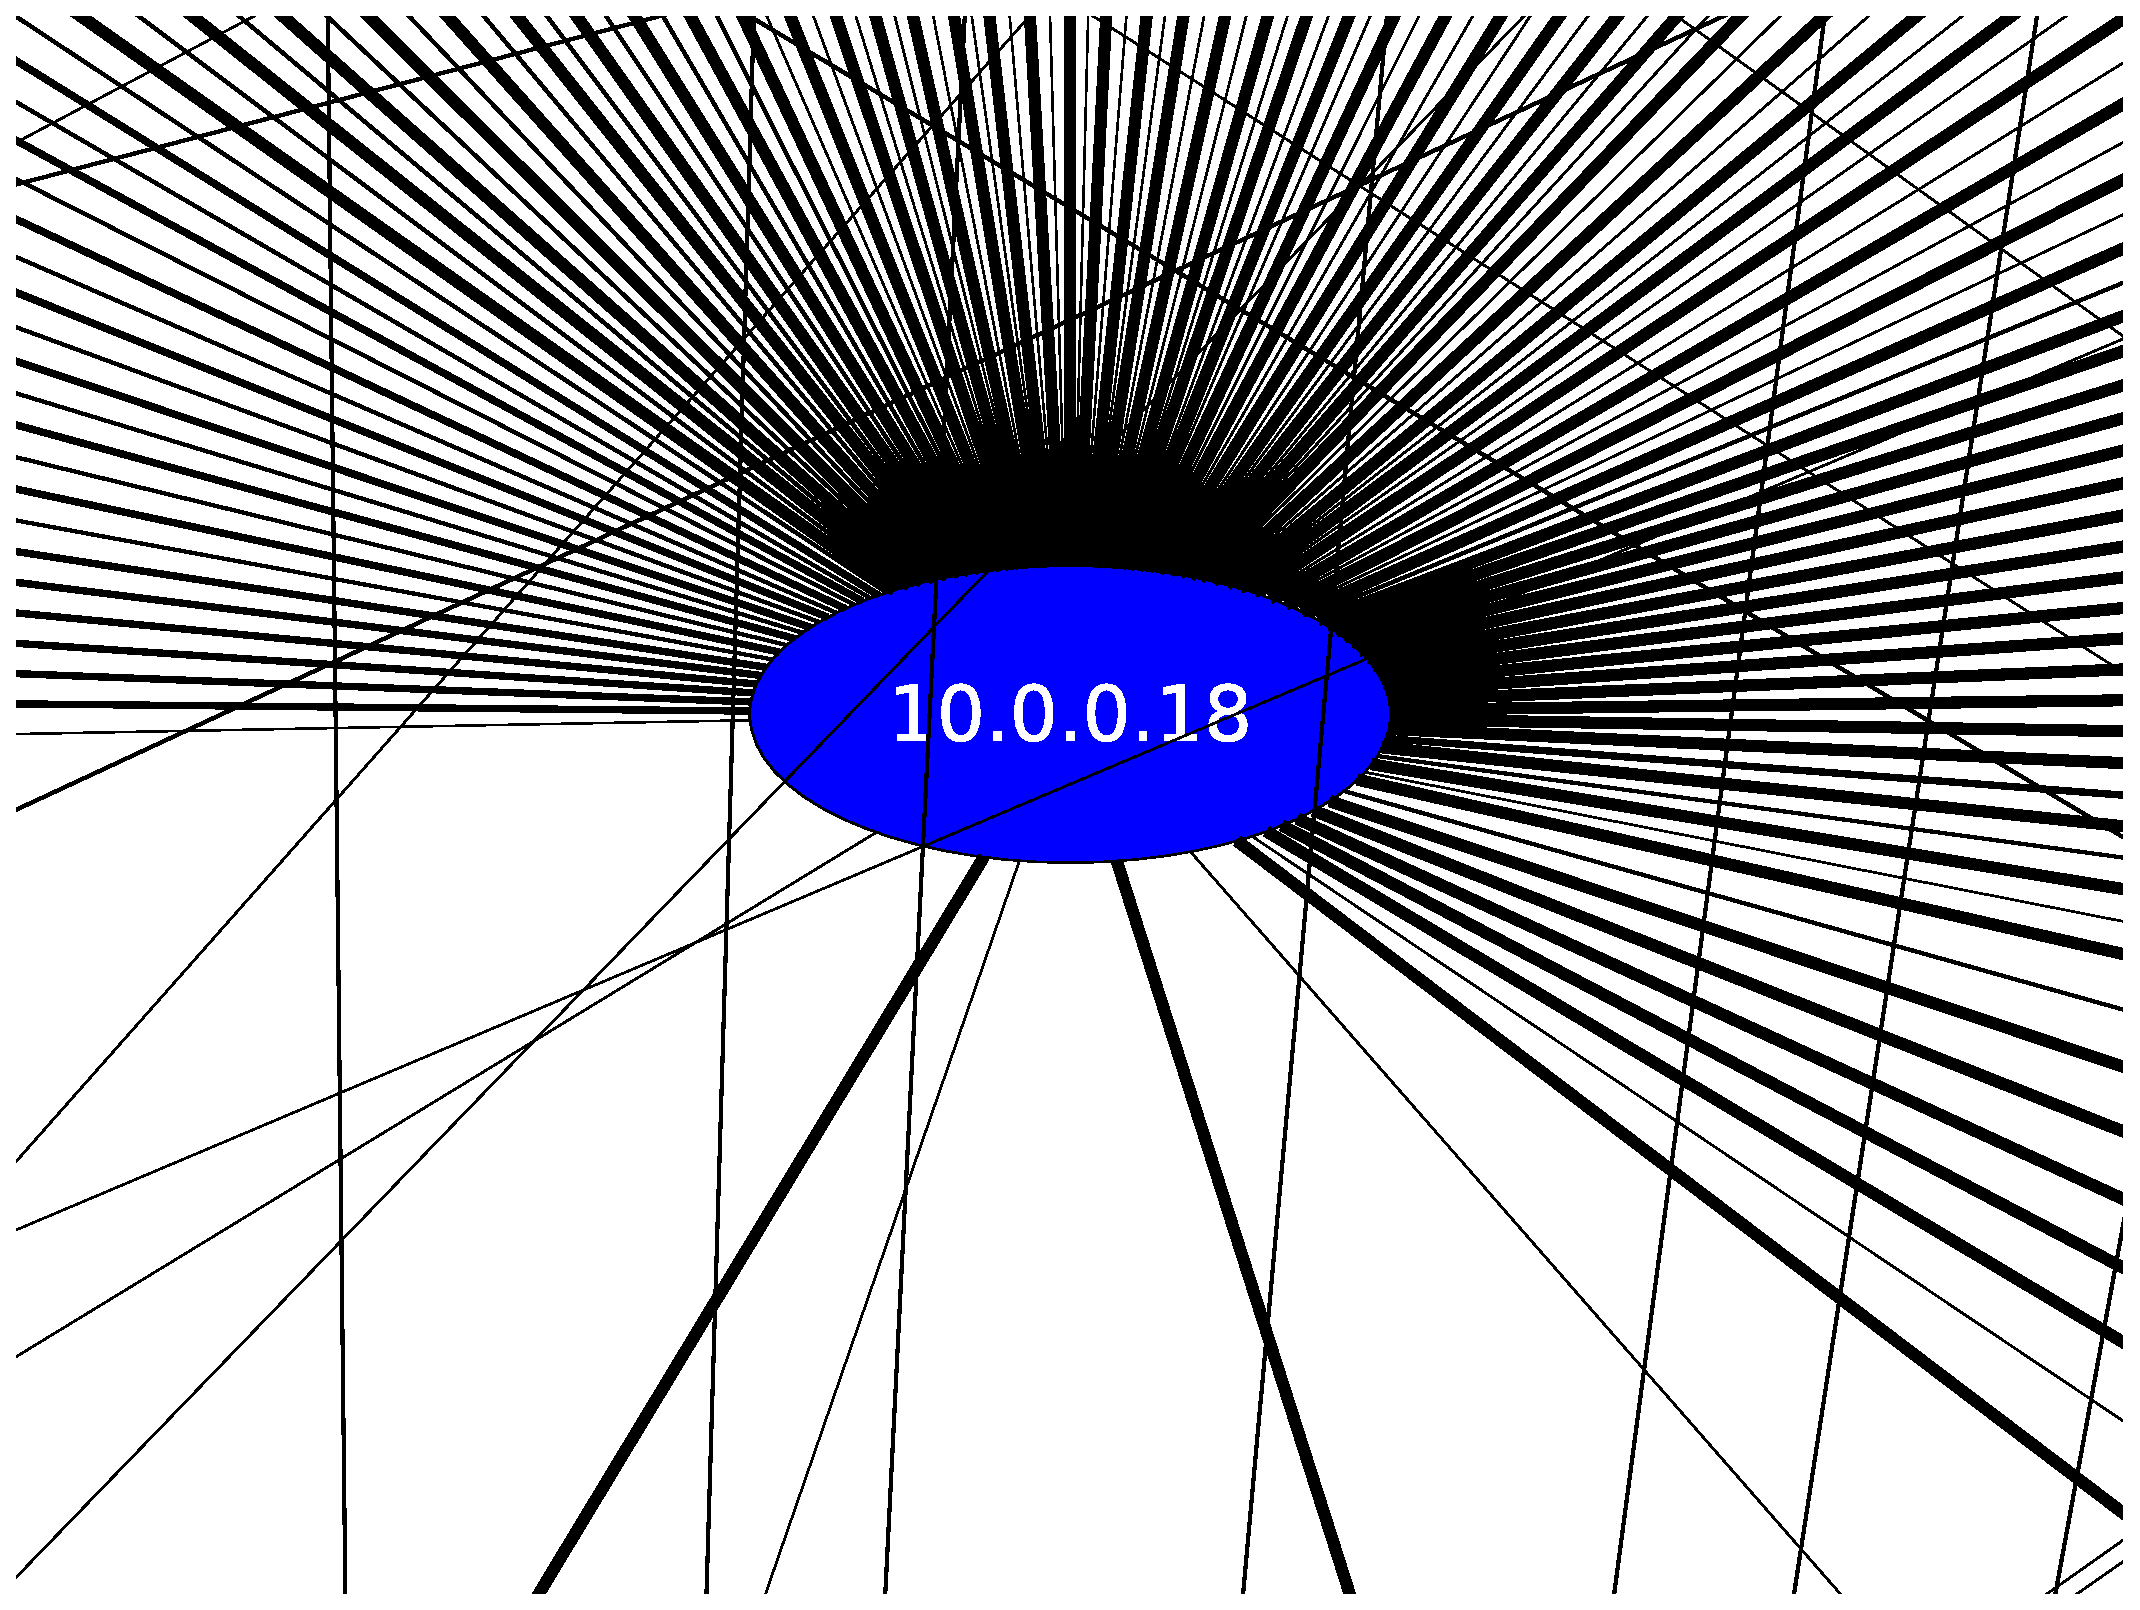
\includegraphics[width=0.5\textwidth]{img/graph/escenario_1/vlan1/vlan1_1000toEnd_10_0_0_18}
    \caption{VLAN \nameref{itm:vlan1} - 10.0.0.18}
    \label{fig:vlan1_grafo_10_0_0_18}
\end{figure}

\begin{figure}[!ht]
    \centering
    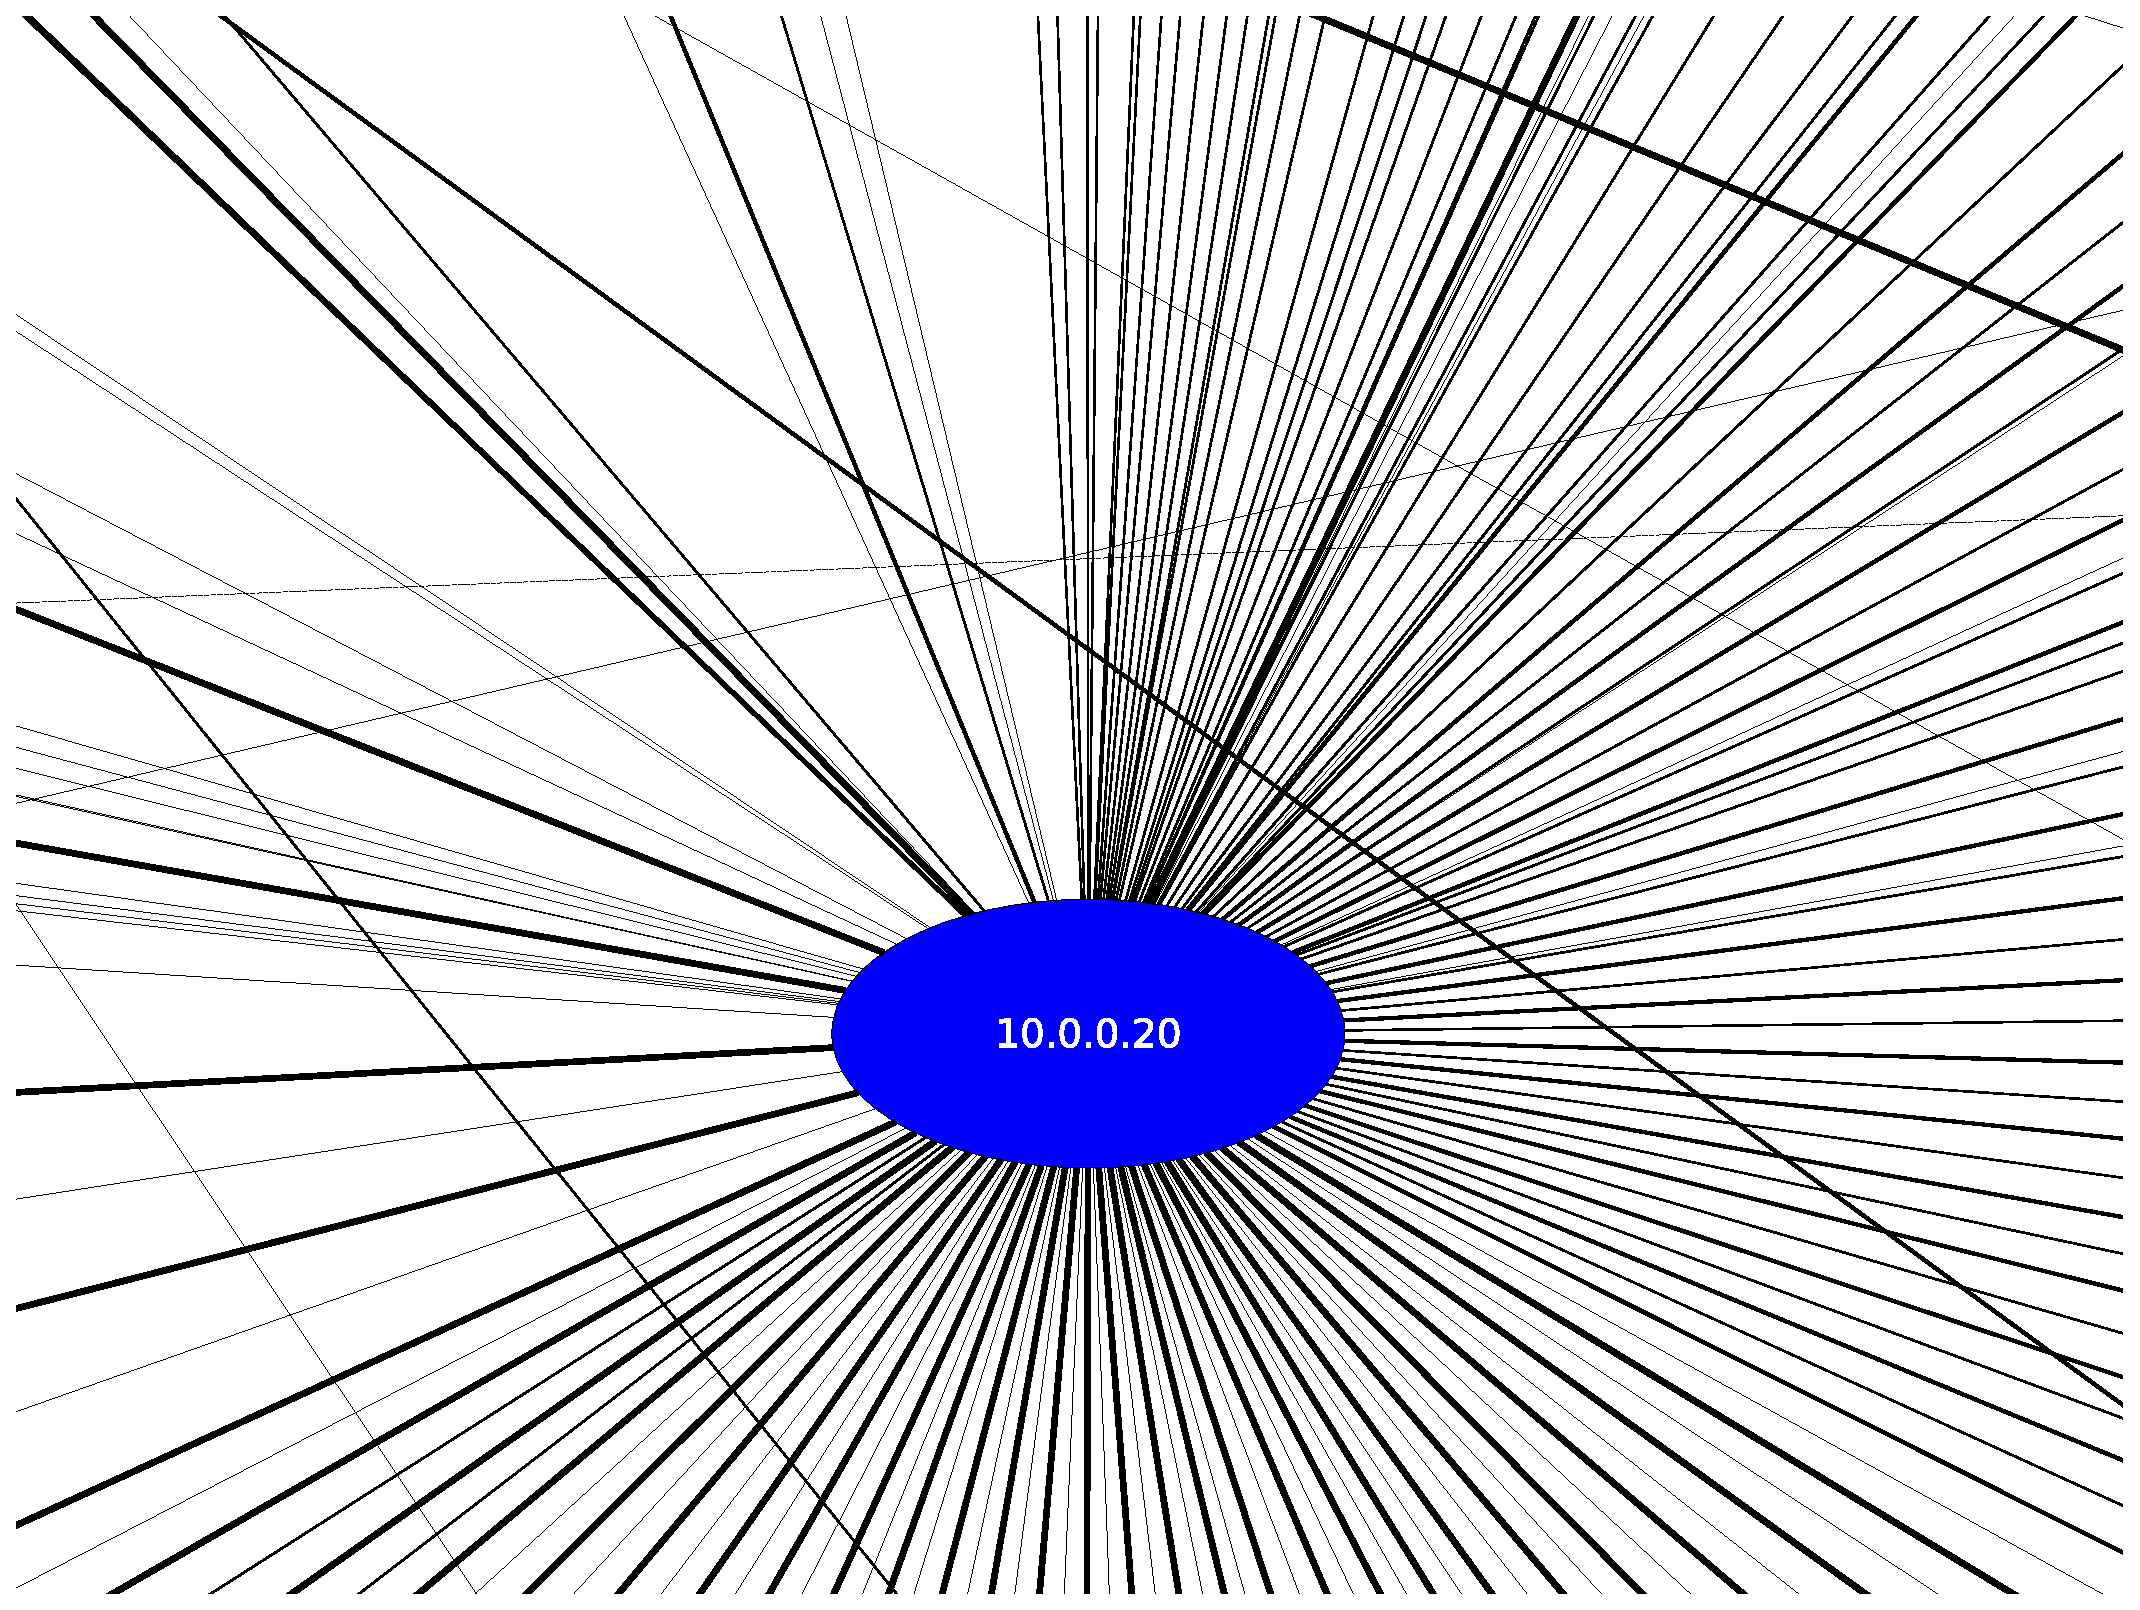
\includegraphics[width=0.5\textwidth]{img/graph/escenario_1/vlan1/vlan1_1000toEnd_10_0_0_20}
    \caption{VLAN \nameref{itm:vlan1} - 10.0.0.20}
    \label{fig:vlan1_grafo_10_0_0_20}
\end{figure}

\par Nos posicionamos ahora sobre la figura \ref{fig:vlan1_grafo_10_2_1_51}, donde se puede
ver que el nodo central no es un nodo azul ni rojo (aquellos nodos marcados por tener una
alta probabilidad en alguna de las dos fuentes de informaci\'on). Aqu\'i se puede observar dicho
host no solo recibe peticiones ARP de sus nodos circundantes, sino que tambi\'en env\'ia \'el
mismo sus propios paquetes del protocolo. As\'i pues, observamos que los nodos que lo rodean
tampoco tienen una gran interacci\'on, salvo alguna excepcion, con el resto de los nodos
\textit{alejados} de la red\footnote{El concepto de \textit{cercan\'ia} es meramente gr\'afico,
e incluso por ah\'i puede aplicar a la red, ya que claramente estos nodos env\'ian paquetes
ARP a el nodo central con frecuencia considerable y no as\'i a otras direcciones \textit{alejadas}
de la red.}. As\'i pues, podemos suponer que esta IP se encarga de ofrecerle alg\'un tipo
de servicio a las terminales que tratan de resolver su \textit{MAC}.

\par Siguiendo en esta figura, se observan las IPs \textit{10.1.254.1, 10.2.13.202 y
10.1.97.101} reciben mayormente conexiones de los nodos de menor tama\~no de esta figura.
Se podr\'ia llegar a suponer que estas direcciones son pose\'idas por hosts que ofrecen
alg\'un tipo de servicio que no requiera ser iniciado por ellos mismos, como por ejemplo,
una base de datos.

\begin{figure}[!htb]
    \centering
    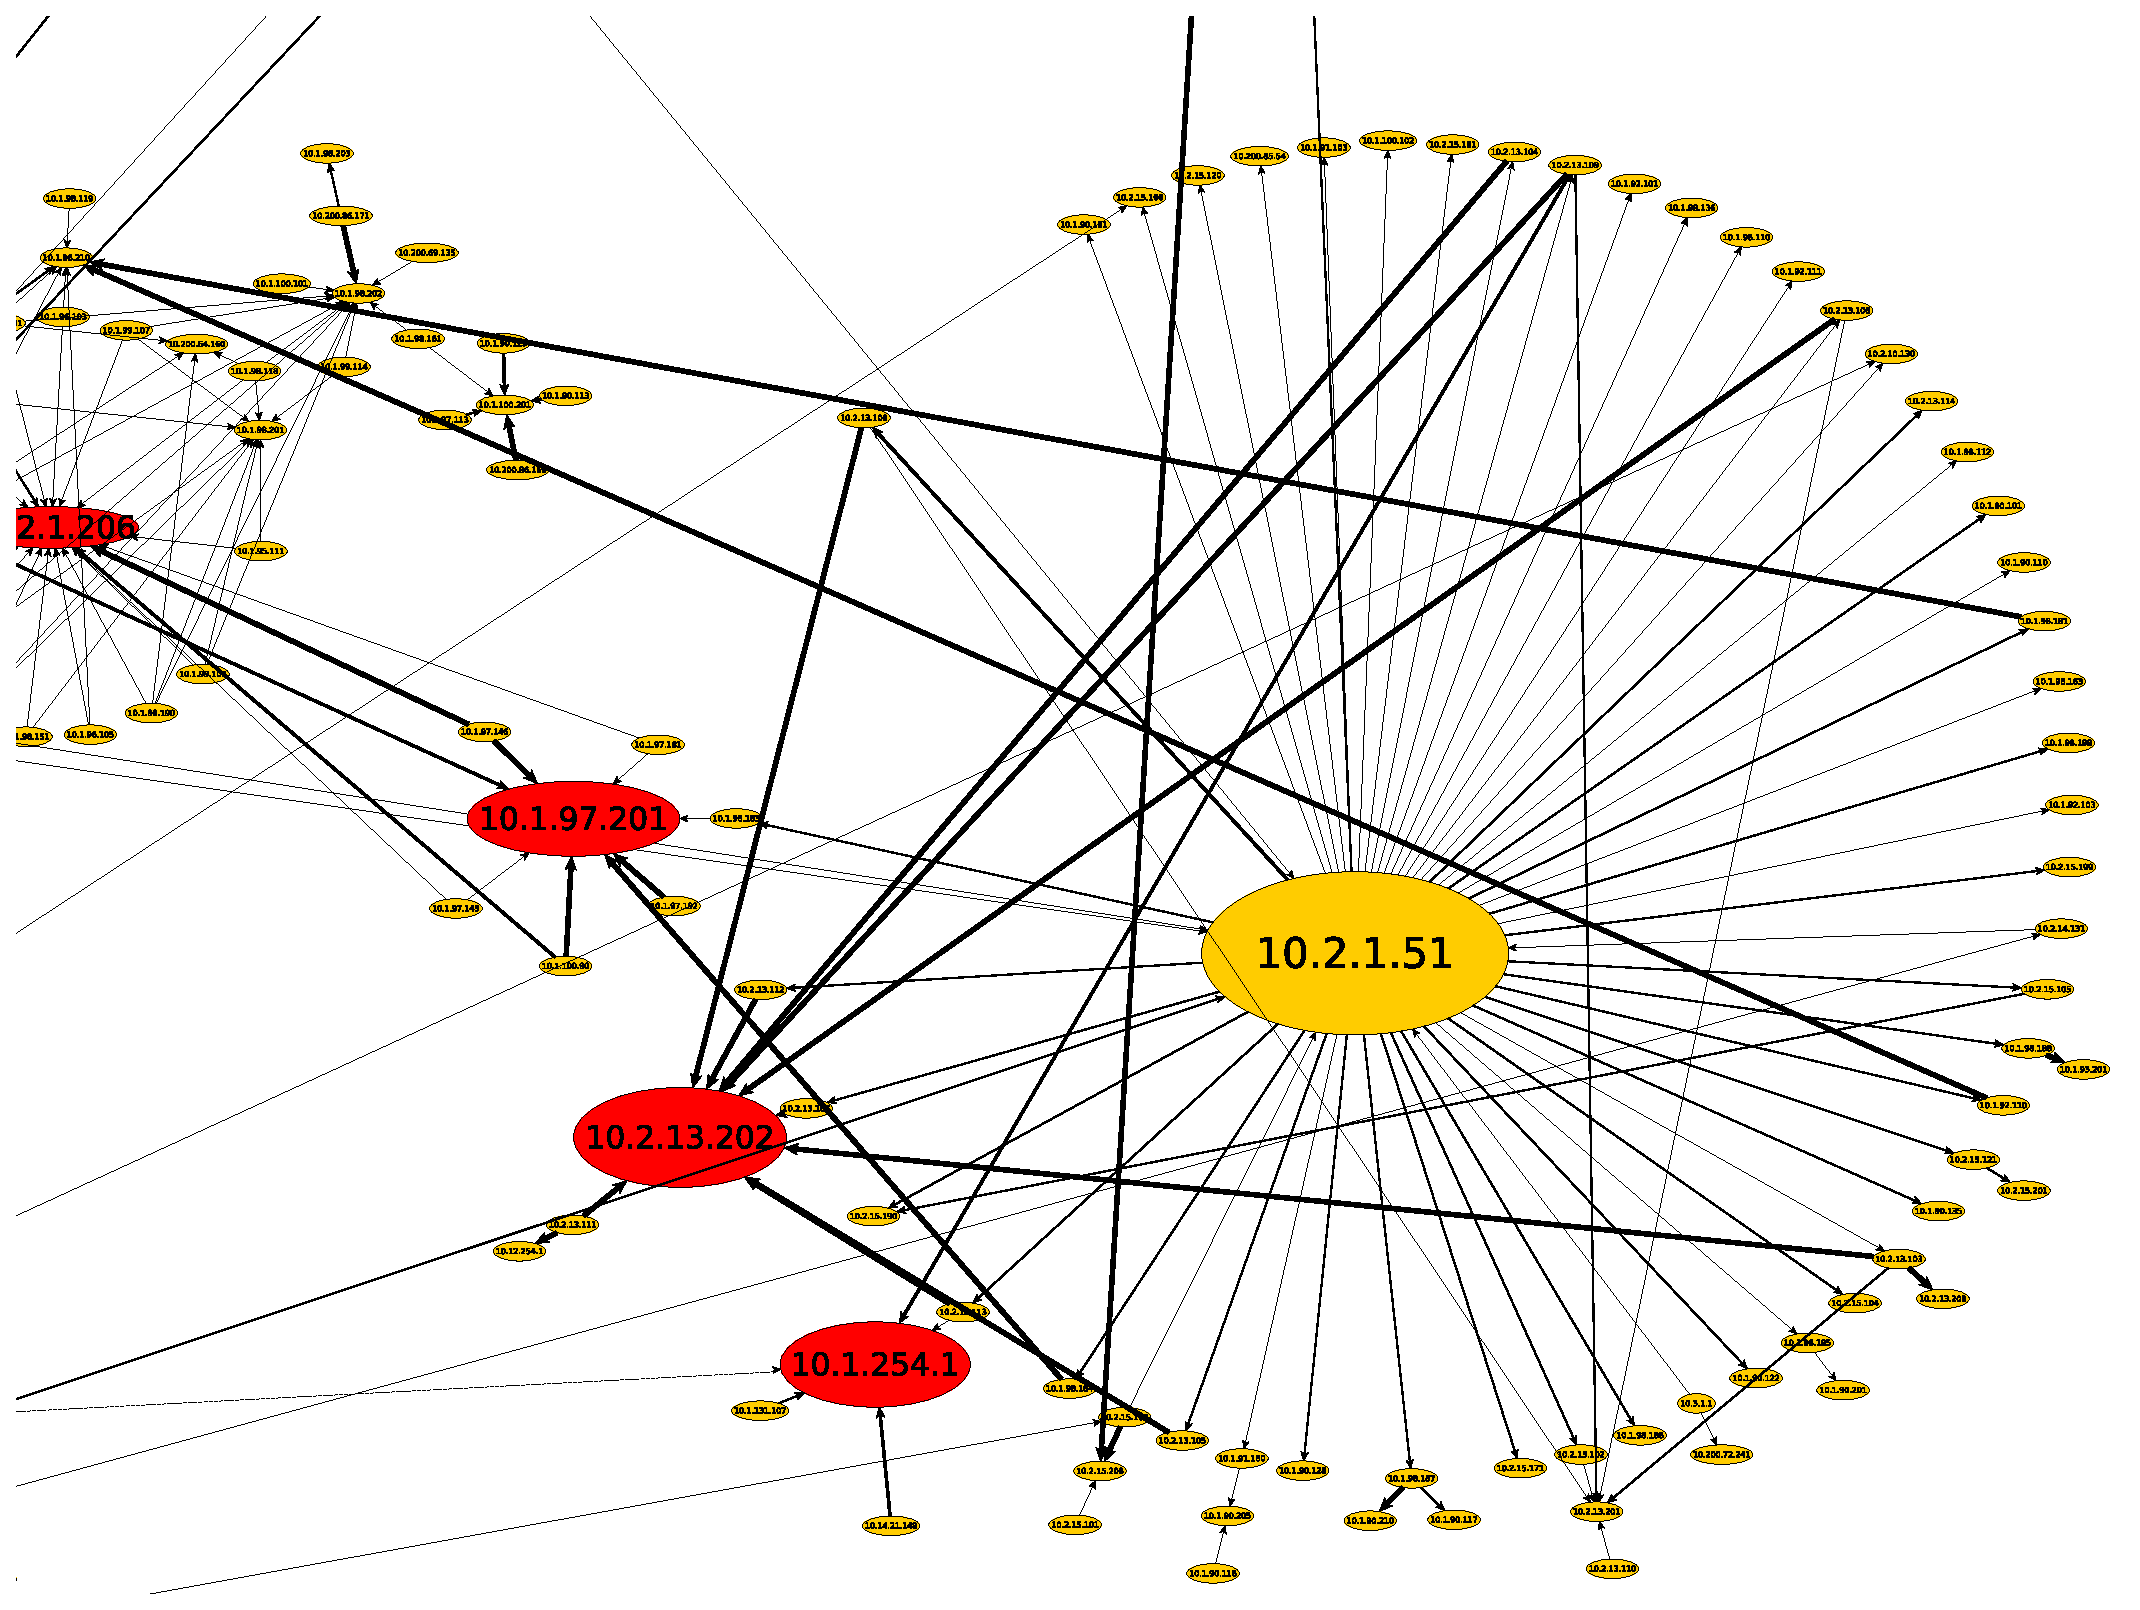
\includegraphics[width=0.5\textwidth]{img/graph/escenario_1/vlan1/vlan1_1000toEnd_10_2_1_51}
    \caption{VLAN \nameref{itm:vlan1} - 10.2.1.51}
    \label{fig:vlan1_grafo_10_2_1_51}
\end{figure}

\par En la misma l\'inea, se aplica lo reci\'en dicho a las figuras \ref{fig:vlan1_grafo_10_2_1_206},
\ref{fig:vlan1_grafo_10_1_254_5} y \ref{fig:vlan1_grafo_10_200_0_44} donde se obserba
el mismo tipo de grafo y comportamiento.

\begin{figure}[!htb]
    \centering
    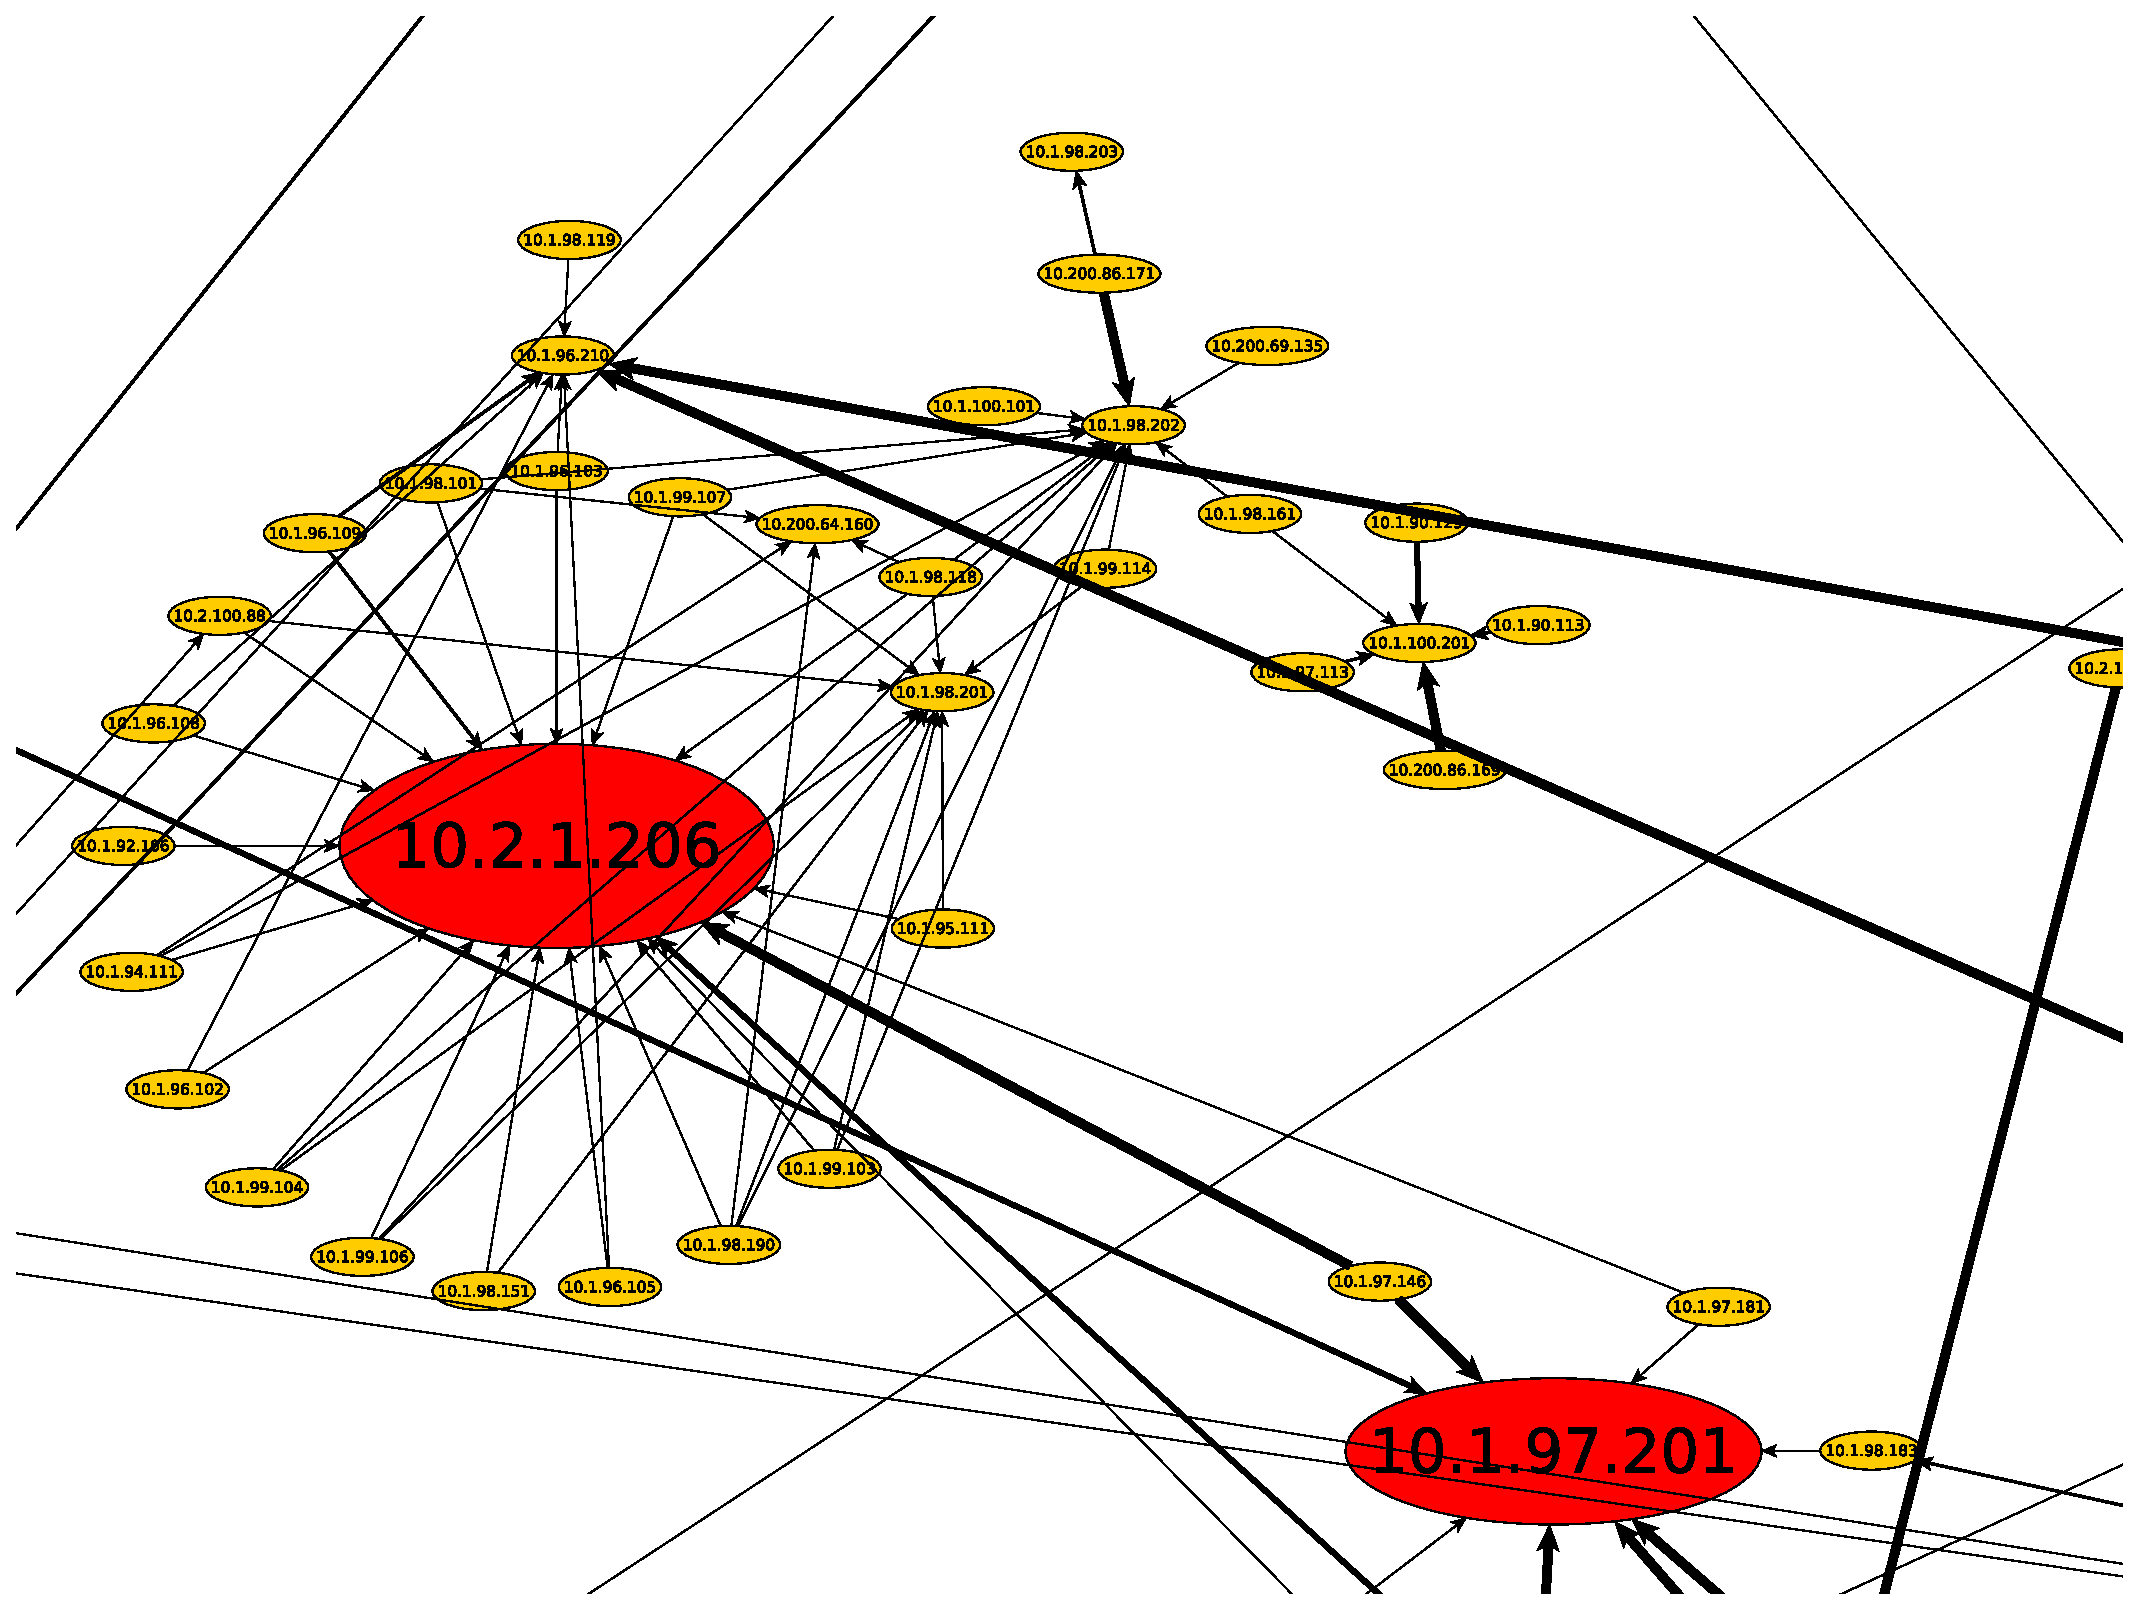
\includegraphics[width=0.5\textwidth]{img/graph/escenario_1/vlan1/vlan1_1000toEnd_10_2_1_206}
    \caption{VLAN \nameref{itm:vlan1} - 10.2.1.206}
    \label{fig:vlan1_grafo_10_2_1_206}
\end{figure}

\begin{figure*}
    \centering
    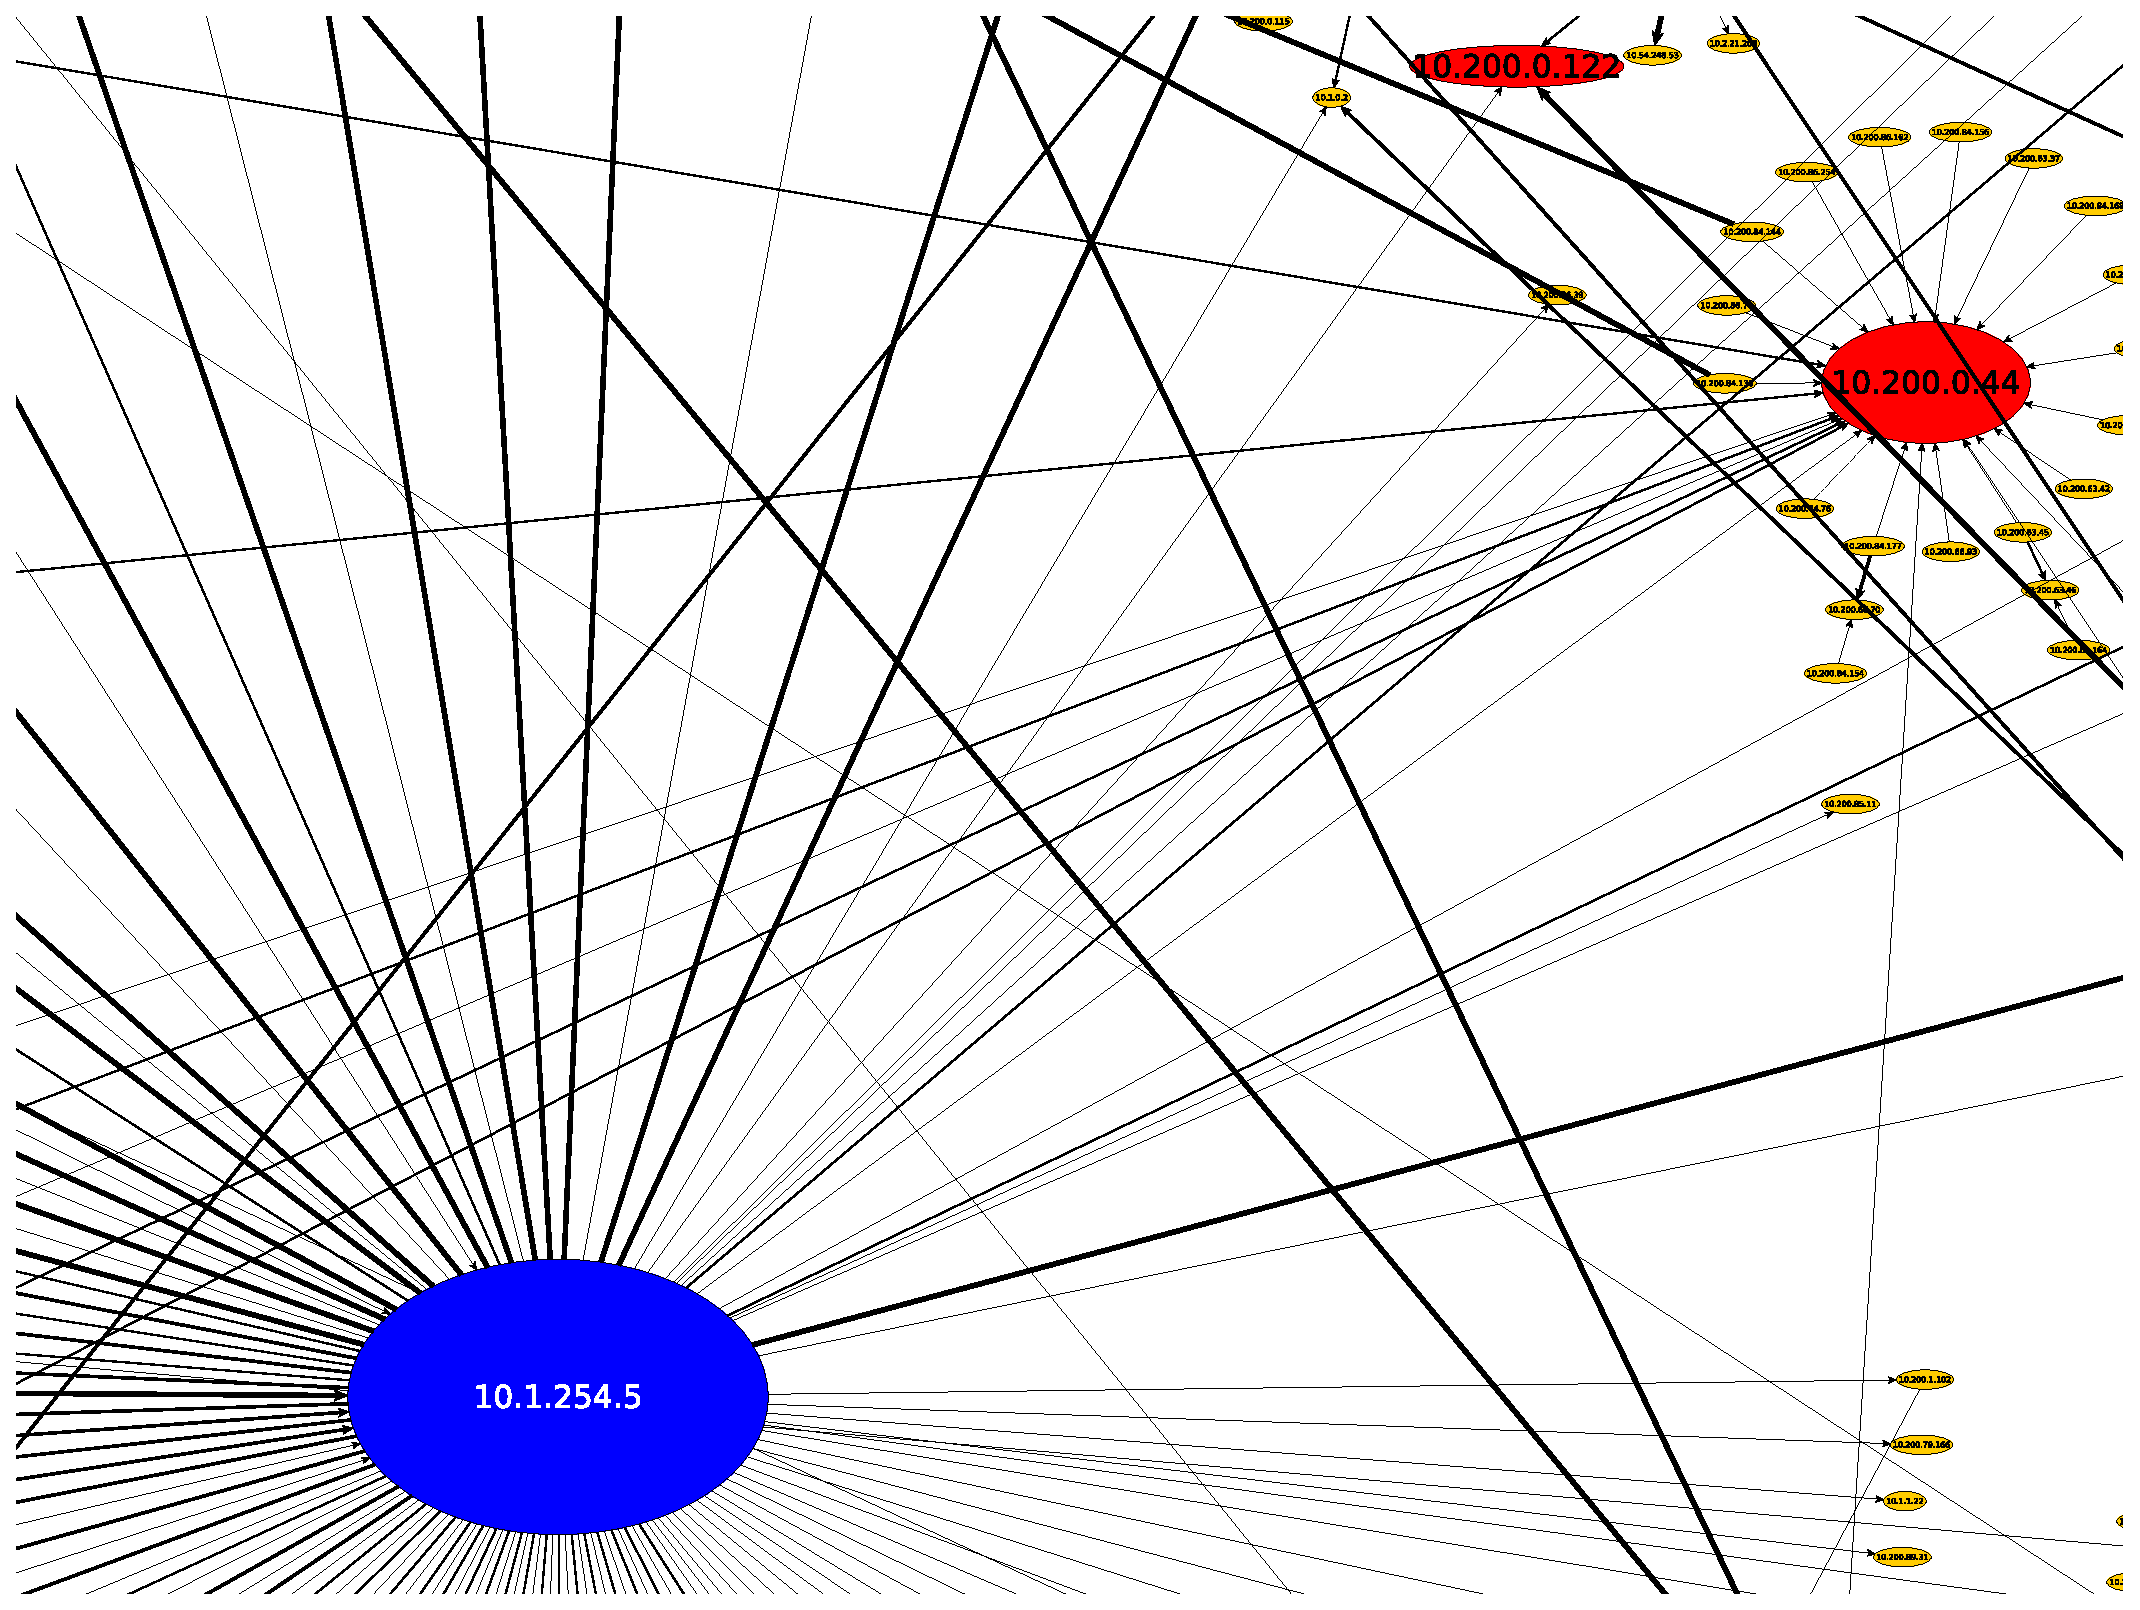
\includegraphics[width=\textwidth]{img/graph/escenario_1/vlan1/vlan1_1000toEnd_10_1_254_5}
    \caption{VLAN \nameref{itm:vlan1} - 10.1.254.5}
    \label{fig:vlan1_grafo_10_1_254_5}
\end{figure*}

\begin{figure}[!ht]
    \centering
    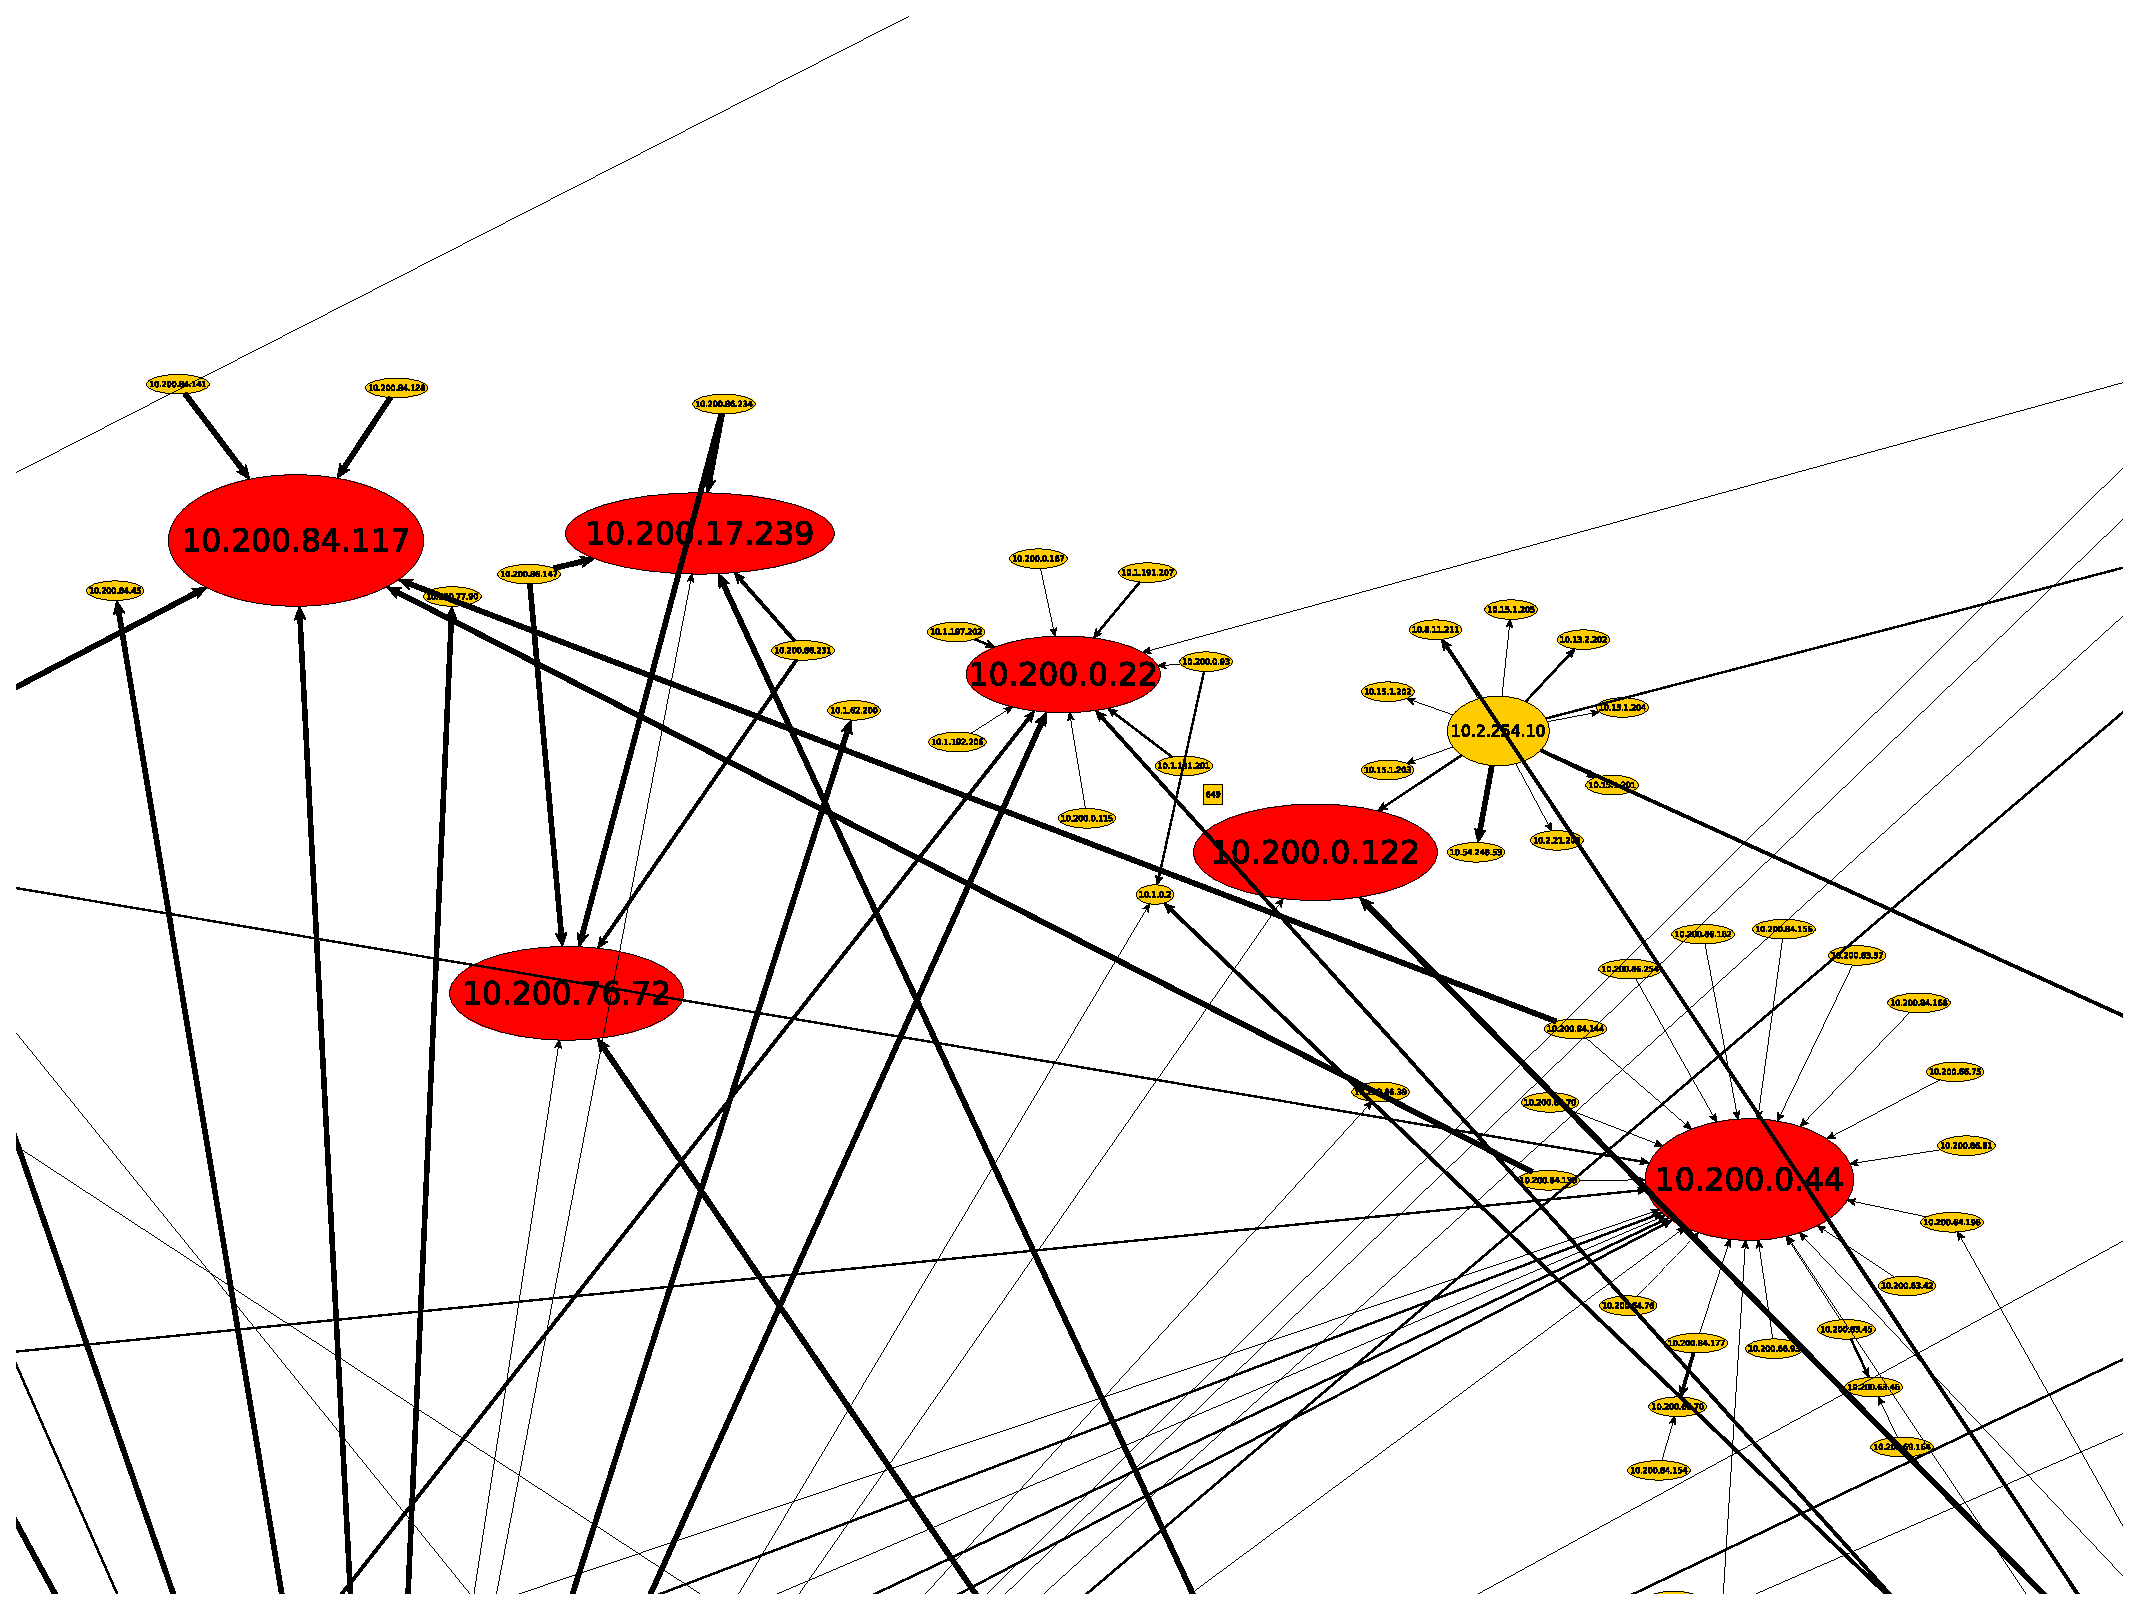
\includegraphics[width=0.5\textwidth]{img/graph/escenario_1/vlan1/vlan1_1000toEnd_10_200_0_44}
    \caption{VLAN \nameref{itm:vlan1} - 10.200.0.44}
    \label{fig:vlan1_grafo_10_200_0_44}
\end{figure}

\FloatBarrier


    %-------------------------------------------------------------------------------------

    \subsection{An\'alisis suplementarios}\label{sec:escenario1_supl}

    \subsection{Conclusiones Preliminares}
